\documentclass{book}
\usepackage[a4paper,top=2.5cm,bottom=2.5cm,left=2.5cm,right=2.5cm]{geometry}
\usepackage{makeidx}
\usepackage{natbib}
\usepackage{graphicx}
\usepackage{multicol}
\usepackage{float}
\usepackage{listings}
\usepackage{color}
\usepackage{ifthen}
\usepackage[table]{xcolor}
\usepackage{textcomp}
\usepackage{alltt}
\usepackage{ifpdf}
\ifpdf
\usepackage[pdftex,
            pagebackref=true,
            colorlinks=true,
            linkcolor=blue,
            unicode
           ]{hyperref}
\else
\usepackage[ps2pdf,
            pagebackref=true,
            colorlinks=true,
            linkcolor=blue,
            unicode
           ]{hyperref}
\usepackage{pspicture}
\fi
\usepackage[utf8]{inputenc}
\usepackage{mathptmx}
\usepackage[scaled=.90]{helvet}
\usepackage{courier}
\usepackage{sectsty}
\usepackage{amssymb}
\usepackage[titles]{tocloft}
\usepackage{doxygen}
\lstset{language=C++,inputencoding=utf8,basicstyle=\footnotesize,breaklines=true,breakatwhitespace=true,tabsize=2,numbers=left }
\makeindex
\setcounter{tocdepth}{3}
\renewcommand{\footrulewidth}{0.4pt}
\renewcommand{\familydefault}{\sfdefault}
\hfuzz=15pt
\setlength{\emergencystretch}{15pt}
\hbadness=750
\tolerance=750
\begin{document}
\hypersetup{pageanchor=false,citecolor=blue}
\begin{titlepage}
\vspace*{7cm}
\begin{center}
{\Large C\-B\-G \\[1ex]\large 0.\-1 }\\
\vspace*{1cm}
{\large Generated by Doxygen 1.8.3.1}\\
\vspace*{0.5cm}
{\small Mon Apr 15 2013 17:43:27}\\
\end{center}
\end{titlepage}
\clearemptydoublepage
\pagenumbering{roman}
\tableofcontents
\clearemptydoublepage
\pagenumbering{arabic}
\hypersetup{pageanchor=true,citecolor=blue}
\chapter{Declaration}
\label{md_DECLARATION}
\hypertarget{md_DECLARATION}{}
We the undersigned declare that the project material, which we now submit, is our own work. Any assistance received by way of borrowing from the work of others has been cited and acknowledged within the work. We make this declaration in the knowledge that a breach of the rules pertaining to project submission may carry serious consequences. We are aware that the project will not be accepted unless this form has been handed in along with the project. 
\chapter{Compendium of board games}
\label{md_README}
\hypertarget{md_README}{}
This is a compendium of four board games wrote in C++.

The games are as follows\-: \hyperlink{classCheckers}{Checkers}, \hyperlink{classConnectFour}{Connect\-Four}, \hyperlink{classSnakesAndLadders}{Snakes\-And\-Ladders} and Reversi. 
\chapter{Hierarchical Index}
\section{Class Hierarchy}
This inheritance list is sorted roughly, but not completely, alphabetically\-:\begin{DoxyCompactList}
\item \contentsline{section}{Coordinate}{\pageref{structCoordinate}}{}
\item \contentsline{section}{Game}{\pageref{classGame}}{}
\begin{DoxyCompactList}
\item \contentsline{section}{Checkers}{\pageref{classCheckers}}{}
\item \contentsline{section}{Connect\-Four}{\pageref{classConnectFour}}{}
\item \contentsline{section}{Snakes\-And\-Ladders}{\pageref{classSnakesAndLadders}}{}
\end{DoxyCompactList}
\item \contentsline{section}{Piece}{\pageref{classPiece}}{}
\begin{DoxyCompactList}
\item \contentsline{section}{Destination\-Piece}{\pageref{classDestinationPiece}}{}
\begin{DoxyCompactList}
\item \contentsline{section}{System\-Piece}{\pageref{classSystemPiece}}{}
\end{DoxyCompactList}
\item \contentsline{section}{Identifier\-Piece}{\pageref{classIdentifierPiece}}{}
\begin{DoxyCompactList}
\item \contentsline{section}{System\-Piece}{\pageref{classSystemPiece}}{}
\end{DoxyCompactList}
\item \contentsline{section}{Source\-Piece}{\pageref{classSourcePiece}}{}
\begin{DoxyCompactList}
\item \contentsline{section}{System\-Piece}{\pageref{classSystemPiece}}{}
\end{DoxyCompactList}
\end{DoxyCompactList}
\item \contentsline{section}{Player}{\pageref{classPlayer}}{}
\begin{DoxyCompactList}
\item \contentsline{section}{Snakes\-And\-Ladders\-Player}{\pageref{classSnakesAndLaddersPlayer}}{}
\end{DoxyCompactList}
\item \contentsline{section}{Square}{\pageref{classSquare}}{}
\end{DoxyCompactList}

\chapter{Data Structure Index}
\section{Data Structures}
Here are the data structures with brief descriptions\-:\begin{DoxyCompactList}
\item\contentsline{section}{\hyperlink{classCheckers}{Checkers} }{\pageref{classCheckers}}{}
\item\contentsline{section}{\hyperlink{classConnectFour}{Connect\-Four} }{\pageref{classConnectFour}}{}
\item\contentsline{section}{\hyperlink{structCoordinate}{Coordinate} }{\pageref{structCoordinate}}{}
\item\contentsline{section}{\hyperlink{classDestinationPiece}{Destination\-Piece} }{\pageref{classDestinationPiece}}{}
\item\contentsline{section}{\hyperlink{classGame}{Game} }{\pageref{classGame}}{}
\item\contentsline{section}{\hyperlink{classIdentifierPiece}{Identifier\-Piece} }{\pageref{classIdentifierPiece}}{}
\item\contentsline{section}{\hyperlink{classPiece}{Piece} }{\pageref{classPiece}}{}
\item\contentsline{section}{\hyperlink{classPlayer}{Player} }{\pageref{classPlayer}}{}
\item\contentsline{section}{\hyperlink{classSnakesAndLadders}{Snakes\-And\-Ladders} }{\pageref{classSnakesAndLadders}}{}
\item\contentsline{section}{\hyperlink{classSnakesAndLaddersPlayer}{Snakes\-And\-Ladders\-Player} }{\pageref{classSnakesAndLaddersPlayer}}{}
\item\contentsline{section}{\hyperlink{classSourcePiece}{Source\-Piece} }{\pageref{classSourcePiece}}{}
\item\contentsline{section}{\hyperlink{classSquare}{Square} }{\pageref{classSquare}}{}
\item\contentsline{section}{\hyperlink{classSystemPiece}{System\-Piece} }{\pageref{classSystemPiece}}{}
\end{DoxyCompactList}

\chapter{File Index}
\section{File List}
Here is a list of all files with brief descriptions\-:\begin{DoxyCompactList}
\item\contentsline{section}{\hyperlink{Checkers_8cpp}{Checkers.\-cpp} }{\pageref{Checkers_8cpp}}{}
\item\contentsline{section}{\hyperlink{Checkers_8h}{Checkers.\-h} }{\pageref{Checkers_8h}}{}
\item\contentsline{section}{\hyperlink{Colors_8h}{Colors.\-h} }{\pageref{Colors_8h}}{}
\item\contentsline{section}{\hyperlink{ConnectFour_8cpp}{Connect\-Four.\-cpp} }{\pageref{ConnectFour_8cpp}}{}
\item\contentsline{section}{\hyperlink{ConnectFour_8h}{Connect\-Four.\-h} }{\pageref{ConnectFour_8h}}{}
\item\contentsline{section}{\hyperlink{Coordinate_8cpp}{Coordinate.\-cpp} }{\pageref{Coordinate_8cpp}}{}
\item\contentsline{section}{\hyperlink{Coordinate_8h}{Coordinate.\-h} }{\pageref{Coordinate_8h}}{}
\item\contentsline{section}{\hyperlink{DestinationPiece_8cpp}{Destination\-Piece.\-cpp} }{\pageref{DestinationPiece_8cpp}}{}
\item\contentsline{section}{\hyperlink{DestinationPiece_8h}{Destination\-Piece.\-h} }{\pageref{DestinationPiece_8h}}{}
\item\contentsline{section}{\hyperlink{Game_8cpp}{Game.\-cpp} }{\pageref{Game_8cpp}}{}
\item\contentsline{section}{\hyperlink{Game_8h}{Game.\-h} }{\pageref{Game_8h}}{}
\item\contentsline{section}{\hyperlink{IdentifierPiece_8cpp}{Identifier\-Piece.\-cpp} }{\pageref{IdentifierPiece_8cpp}}{}
\item\contentsline{section}{\hyperlink{IdentifierPiece_8h}{Identifier\-Piece.\-h} }{\pageref{IdentifierPiece_8h}}{}
\item\contentsline{section}{\hyperlink{main_8cpp}{main.\-cpp} }{\pageref{main_8cpp}}{}
\item\contentsline{section}{\hyperlink{Piece_8cpp}{Piece.\-cpp} }{\pageref{Piece_8cpp}}{}
\item\contentsline{section}{\hyperlink{Piece_8h}{Piece.\-h} }{\pageref{Piece_8h}}{}
\item\contentsline{section}{\hyperlink{Player_8cpp}{Player.\-cpp} }{\pageref{Player_8cpp}}{}
\item\contentsline{section}{\hyperlink{Player_8h}{Player.\-h} }{\pageref{Player_8h}}{}
\item\contentsline{section}{\hyperlink{SnakesAndLadders_8cpp}{Snakes\-And\-Ladders.\-cpp} }{\pageref{SnakesAndLadders_8cpp}}{}
\item\contentsline{section}{\hyperlink{SnakesAndLadders_8h}{Snakes\-And\-Ladders.\-h} }{\pageref{SnakesAndLadders_8h}}{}
\item\contentsline{section}{\hyperlink{SnakesAndLaddersPlayer_8cpp}{Snakes\-And\-Ladders\-Player.\-cpp} }{\pageref{SnakesAndLaddersPlayer_8cpp}}{}
\item\contentsline{section}{\hyperlink{SnakesAndLaddersPlayer_8h}{Snakes\-And\-Ladders\-Player.\-h} }{\pageref{SnakesAndLaddersPlayer_8h}}{}
\item\contentsline{section}{\hyperlink{SourcePiece_8cpp}{Source\-Piece.\-cpp} }{\pageref{SourcePiece_8cpp}}{}
\item\contentsline{section}{\hyperlink{SourcePiece_8h}{Source\-Piece.\-h} }{\pageref{SourcePiece_8h}}{}
\item\contentsline{section}{\hyperlink{Square_8cpp}{Square.\-cpp} }{\pageref{Square_8cpp}}{}
\item\contentsline{section}{\hyperlink{Square_8h}{Square.\-h} }{\pageref{Square_8h}}{}
\item\contentsline{section}{\hyperlink{SystemPiece_8cpp}{System\-Piece.\-cpp} }{\pageref{SystemPiece_8cpp}}{}
\item\contentsline{section}{\hyperlink{SystemPiece_8h}{System\-Piece.\-h} }{\pageref{SystemPiece_8h}}{}
\end{DoxyCompactList}

\chapter{Data Structure Documentation}
\hypertarget{classCheckers}{\section{Checkers Class Reference}
\label{classCheckers}\index{Checkers@{Checkers}}
}


{\ttfamily \#include $<$Checkers.\-h$>$}

Inheritance diagram for Checkers\-:\begin{figure}[H]
\begin{center}
\leavevmode
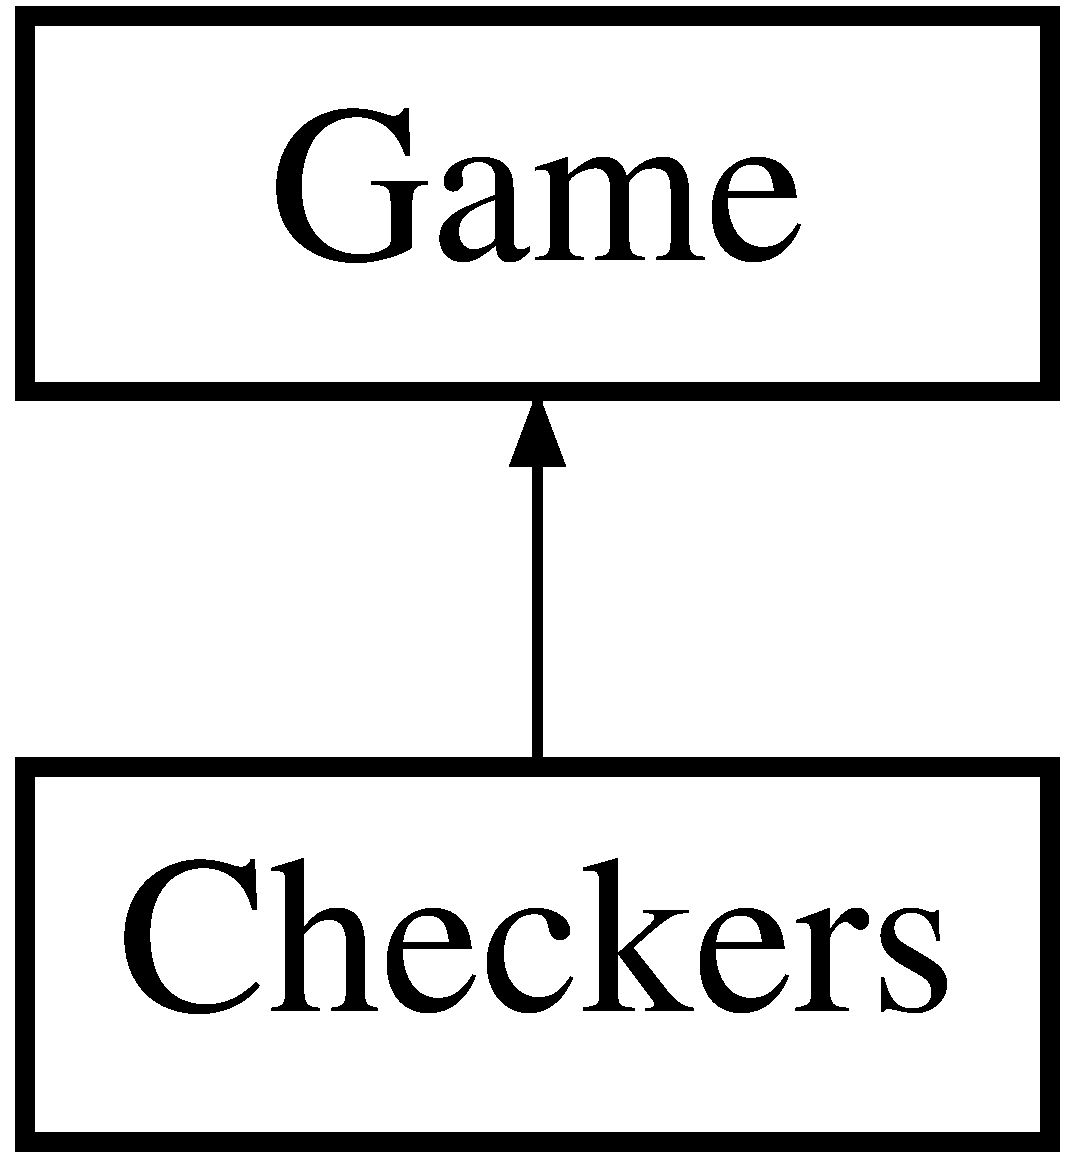
\includegraphics[height=2.000000cm]{classCheckers}
\end{center}
\end{figure}
\subsection*{Public Member Functions}
\begin{DoxyCompactItemize}
\item 
\hyperlink{classCheckers_aac46ea0bb5bdeb648d59710785633838}{Checkers} ()
\end{DoxyCompactItemize}
\subsection*{Additional Inherited Members}


\subsection{Detailed Description}
\hyperlink{classCheckers}{Checkers} \hyperlink{classGame}{Game}. \begin{DoxyAuthor}{Author}
Ian Duffy 
\end{DoxyAuthor}


Definition at line 9 of file Checkers.\-h.



\subsection{Constructor \& Destructor Documentation}
\hypertarget{classCheckers_aac46ea0bb5bdeb648d59710785633838}{\index{Checkers@{Checkers}!Checkers@{Checkers}}
\index{Checkers@{Checkers}!Checkers@{Checkers}}
\subsubsection[{Checkers}]{\setlength{\rightskip}{0pt plus 5cm}Checkers\-::\-Checkers (
\begin{DoxyParamCaption}
{}
\end{DoxyParamCaption}
)}}\label{classCheckers_aac46ea0bb5bdeb648d59710785633838}


Definition at line 11 of file Checkers.\-cpp.



The documentation for this class was generated from the following files\-:\begin{DoxyCompactItemize}
\item 
\hyperlink{Checkers_8h}{Checkers.\-h}\item 
\hyperlink{Checkers_8cpp}{Checkers.\-cpp}\end{DoxyCompactItemize}

\hypertarget{classConnectFour}{\section{Connect\-Four Class Reference}
\label{classConnectFour}\index{Connect\-Four@{Connect\-Four}}
}


{\ttfamily \#include $<$Connect\-Four.\-h$>$}

Inheritance diagram for Connect\-Four\-:\begin{figure}[H]
\begin{center}
\leavevmode
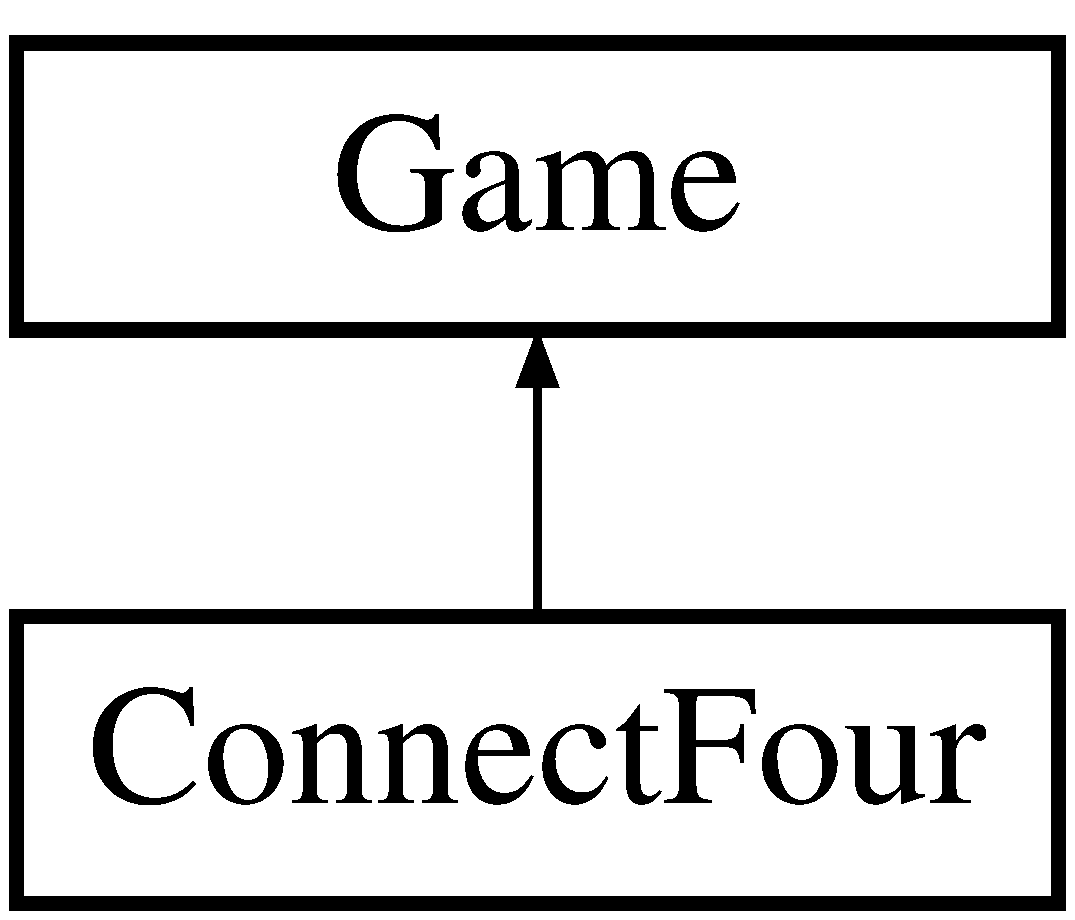
\includegraphics[height=2.000000cm]{classConnectFour}
\end{center}
\end{figure}
\subsection*{Public Member Functions}
\begin{DoxyCompactItemize}
\item 
\hyperlink{classConnectFour_a9d7a0db424f22513386fa60ed2d5b575}{Connect\-Four} ()
\end{DoxyCompactItemize}
\subsection*{Additional Inherited Members}


\subsection{Detailed Description}


Definition at line 12 of file Connect\-Four.\-h.



\subsection{Constructor \& Destructor Documentation}
\hypertarget{classConnectFour_a9d7a0db424f22513386fa60ed2d5b575}{\index{Connect\-Four@{Connect\-Four}!Connect\-Four@{Connect\-Four}}
\index{Connect\-Four@{Connect\-Four}!ConnectFour@{Connect\-Four}}
\subsubsection[{Connect\-Four}]{\setlength{\rightskip}{0pt plus 5cm}Connect\-Four\-::\-Connect\-Four (
\begin{DoxyParamCaption}
{}
\end{DoxyParamCaption}
)}}\label{classConnectFour_a9d7a0db424f22513386fa60ed2d5b575}


Definition at line 8 of file Connect\-Four.\-cpp.



The documentation for this class was generated from the following files\-:\begin{DoxyCompactItemize}
\item 
\hyperlink{ConnectFour_8h}{Connect\-Four.\-h}\item 
\hyperlink{ConnectFour_8cpp}{Connect\-Four.\-cpp}\end{DoxyCompactItemize}

\hypertarget{structCoordinate}{\section{Coordinate Struct Reference}
\label{structCoordinate}\index{Coordinate@{Coordinate}}
}


{\ttfamily \#include $<$Coordinate.\-h$>$}

\subsection*{Public Member Functions}
\begin{DoxyCompactItemize}
\item 
\hyperlink{structCoordinate_aac6f323a685fc1e88fbea9c86f1e600d}{Coordinate} ()
\item 
\hyperlink{structCoordinate_aba3fc03b1a25f335c9058ddf18290d59}{Coordinate} (int \hyperlink{structCoordinate_ad462d671f1feb865911333e3ff5f0a5d}{x}, int \hyperlink{structCoordinate_a5c7d59f0f65ff9371b6c3791f78880aa}{y})
\end{DoxyCompactItemize}
\subsection*{Data Fields}
\begin{DoxyCompactItemize}
\item 
int \hyperlink{structCoordinate_ad462d671f1feb865911333e3ff5f0a5d}{x}
\begin{DoxyCompactList}\small\item\em The X position. \end{DoxyCompactList}\item 
int \hyperlink{structCoordinate_a5c7d59f0f65ff9371b6c3791f78880aa}{y}
\begin{DoxyCompactList}\small\item\em The Y position. \end{DoxyCompactList}\end{DoxyCompactItemize}


\subsection{Detailed Description}
Encapsulates the idea of a location made up of an X point and a Y point. \begin{DoxyAuthor}{Author}
Darren Brogan 
\end{DoxyAuthor}


Definition at line 7 of file Coordinate.\-h.



\subsection{Constructor \& Destructor Documentation}
\hypertarget{structCoordinate_aac6f323a685fc1e88fbea9c86f1e600d}{\index{Coordinate@{Coordinate}!Coordinate@{Coordinate}}
\index{Coordinate@{Coordinate}!Coordinate@{Coordinate}}
\subsubsection[{Coordinate}]{\setlength{\rightskip}{0pt plus 5cm}Coordinate\-::\-Coordinate (
\begin{DoxyParamCaption}
{}
\end{DoxyParamCaption}
)}}\label{structCoordinate_aac6f323a685fc1e88fbea9c86f1e600d}
Encapsulates the idea of a location made up of an X point and a Y point. \begin{DoxyAuthor}{Author}
Darren Brogan 
\end{DoxyAuthor}


Definition at line 6 of file Coordinate.\-cpp.

\hypertarget{structCoordinate_aba3fc03b1a25f335c9058ddf18290d59}{\index{Coordinate@{Coordinate}!Coordinate@{Coordinate}}
\index{Coordinate@{Coordinate}!Coordinate@{Coordinate}}
\subsubsection[{Coordinate}]{\setlength{\rightskip}{0pt plus 5cm}Coordinate\-::\-Coordinate (
\begin{DoxyParamCaption}
\item[{int}]{x, }
\item[{int}]{y}
\end{DoxyParamCaption}
)}}\label{structCoordinate_aba3fc03b1a25f335c9058ddf18290d59}


Definition at line 8 of file Coordinate.\-cpp.



\subsection{Field Documentation}
\hypertarget{structCoordinate_ad462d671f1feb865911333e3ff5f0a5d}{\index{Coordinate@{Coordinate}!x@{x}}
\index{x@{x}!Coordinate@{Coordinate}}
\subsubsection[{x}]{\setlength{\rightskip}{0pt plus 5cm}int Coordinate\-::x}}\label{structCoordinate_ad462d671f1feb865911333e3ff5f0a5d}


The X position. 



Definition at line 9 of file Coordinate.\-h.

\hypertarget{structCoordinate_a5c7d59f0f65ff9371b6c3791f78880aa}{\index{Coordinate@{Coordinate}!y@{y}}
\index{y@{y}!Coordinate@{Coordinate}}
\subsubsection[{y}]{\setlength{\rightskip}{0pt plus 5cm}int Coordinate\-::y}}\label{structCoordinate_a5c7d59f0f65ff9371b6c3791f78880aa}


The Y position. 



Definition at line 12 of file Coordinate.\-h.



The documentation for this struct was generated from the following files\-:\begin{DoxyCompactItemize}
\item 
\hyperlink{Coordinate_8h}{Coordinate.\-h}\item 
\hyperlink{Coordinate_8cpp}{Coordinate.\-cpp}\end{DoxyCompactItemize}

\hypertarget{classDestinationPiece}{\section{Destination\-Piece Class Reference}
\label{classDestinationPiece}\index{Destination\-Piece@{Destination\-Piece}}
}


{\ttfamily \#include $<$Destination\-Piece.\-h$>$}

Inheritance diagram for Destination\-Piece\-:\begin{figure}[H]
\begin{center}
\leavevmode
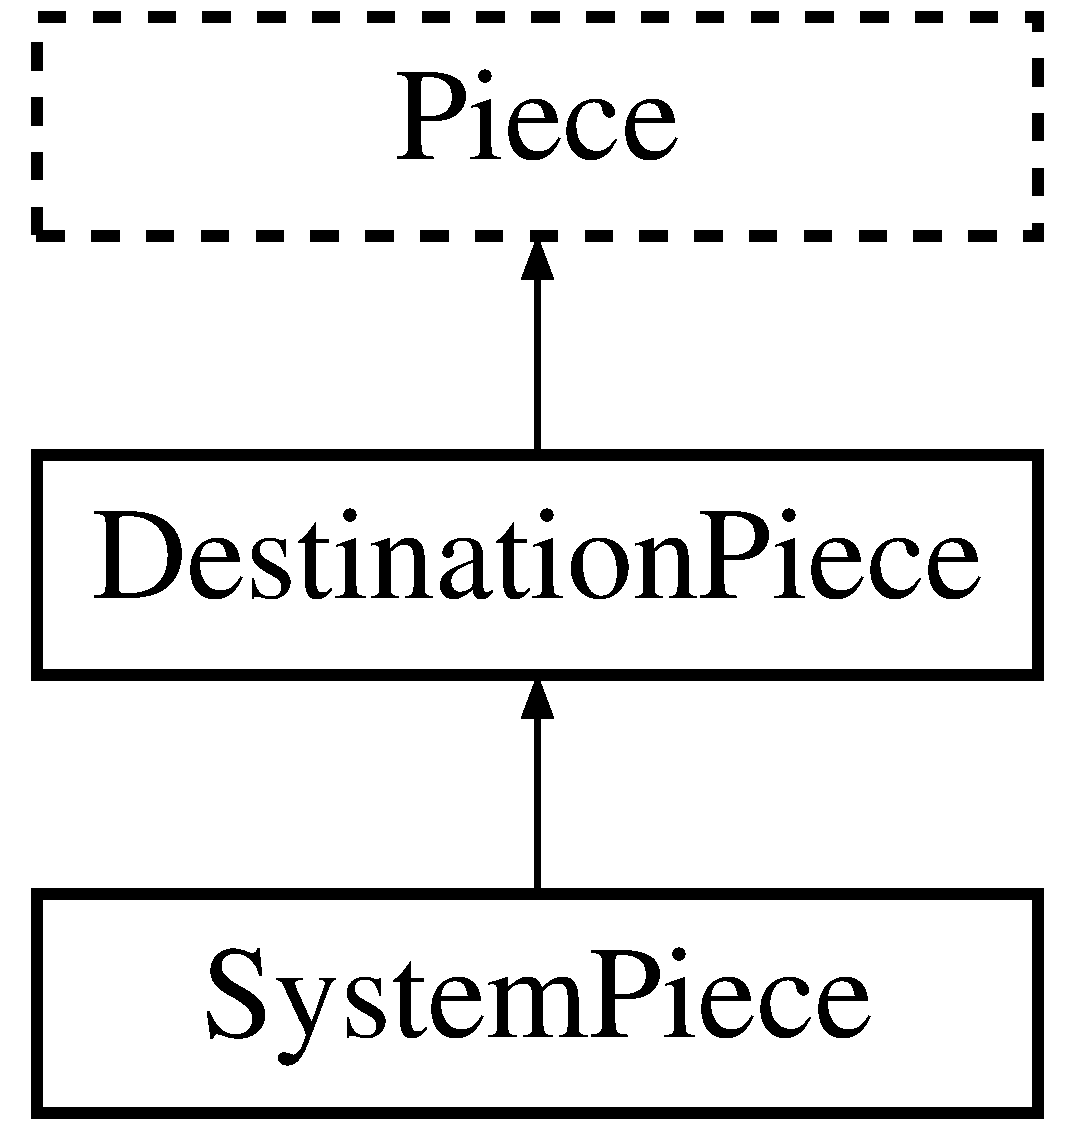
\includegraphics[height=3.000000cm]{classDestinationPiece}
\end{center}
\end{figure}
\subsection*{Public Member Functions}
\begin{DoxyCompactItemize}
\item 
\hyperlink{classDestinationPiece_a6157318c1a312597dafa26c895077ebd}{Destination\-Piece} (\hyperlink{classPlayer}{Player} $\ast$\hyperlink{classPiece_a43beac3b5268343b9f7e575d637eda98}{owner}, \hyperlink{structCoordinate}{Coordinate} \hyperlink{classDestinationPiece_acd3a864aa8c242f3b8b7d27195a2d879}{destination})
\item 
\hyperlink{structCoordinate}{Coordinate} \hyperlink{classDestinationPiece_a6a6d7885523146bc18730d249060e37c}{get\-Destination} ()
\begin{DoxyCompactList}\small\item\em Returns the destination. \end{DoxyCompactList}\item 
void \hyperlink{classDestinationPiece_af0443c30ba2a07eb060f8b89040f5cd1}{set\-Destination} (\hyperlink{structCoordinate}{Coordinate} \hyperlink{classDestinationPiece_acd3a864aa8c242f3b8b7d27195a2d879}{destination})
\begin{DoxyCompactList}\small\item\em Sets the destination coordinate. \end{DoxyCompactList}\end{DoxyCompactItemize}
\subsection*{Protected Attributes}
\begin{DoxyCompactItemize}
\item 
\hyperlink{structCoordinate}{Coordinate} \hyperlink{classDestinationPiece_acd3a864aa8c242f3b8b7d27195a2d879}{destination}
\begin{DoxyCompactList}\small\item\em \hyperlink{structCoordinate}{Coordinate} containing the destination. \end{DoxyCompactList}\end{DoxyCompactItemize}
\subsection*{Additional Inherited Members}


\subsection{Detailed Description}
A \hyperlink{classPiece}{Piece} with a destination. \begin{DoxyAuthor}{Author}
Ian Duffy 
\end{DoxyAuthor}


Definition at line 9 of file Destination\-Piece.\-h.



\subsection{Constructor \& Destructor Documentation}
\hypertarget{classDestinationPiece_a6157318c1a312597dafa26c895077ebd}{\index{Destination\-Piece@{Destination\-Piece}!Destination\-Piece@{Destination\-Piece}}
\index{Destination\-Piece@{Destination\-Piece}!DestinationPiece@{Destination\-Piece}}
\subsubsection[{Destination\-Piece}]{\setlength{\rightskip}{0pt plus 5cm}Destination\-Piece\-::\-Destination\-Piece (
\begin{DoxyParamCaption}
\item[{{\bf Player} $\ast$}]{owner, }
\item[{{\bf Coordinate}}]{destination}
\end{DoxyParamCaption}
)}}\label{classDestinationPiece_a6157318c1a312597dafa26c895077ebd}
A \hyperlink{classPiece}{Piece} with a destination. \begin{DoxyAuthor}{Author}
Ian Duffy 
\end{DoxyAuthor}


Definition at line 6 of file Destination\-Piece.\-cpp.



\subsection{Member Function Documentation}
\hypertarget{classDestinationPiece_a6a6d7885523146bc18730d249060e37c}{\index{Destination\-Piece@{Destination\-Piece}!get\-Destination@{get\-Destination}}
\index{get\-Destination@{get\-Destination}!DestinationPiece@{Destination\-Piece}}
\subsubsection[{get\-Destination}]{\setlength{\rightskip}{0pt plus 5cm}{\bf Coordinate} Destination\-Piece\-::get\-Destination (
\begin{DoxyParamCaption}
{}
\end{DoxyParamCaption}
)}}\label{classDestinationPiece_a6a6d7885523146bc18730d249060e37c}


Returns the destination. 



Definition at line 12 of file Destination\-Piece.\-cpp.

\hypertarget{classDestinationPiece_af0443c30ba2a07eb060f8b89040f5cd1}{\index{Destination\-Piece@{Destination\-Piece}!set\-Destination@{set\-Destination}}
\index{set\-Destination@{set\-Destination}!DestinationPiece@{Destination\-Piece}}
\subsubsection[{set\-Destination}]{\setlength{\rightskip}{0pt plus 5cm}void Destination\-Piece\-::set\-Destination (
\begin{DoxyParamCaption}
\item[{{\bf Coordinate}}]{destination}
\end{DoxyParamCaption}
)}}\label{classDestinationPiece_af0443c30ba2a07eb060f8b89040f5cd1}


Sets the destination coordinate. 



Definition at line 17 of file Destination\-Piece.\-cpp.



\subsection{Field Documentation}
\hypertarget{classDestinationPiece_acd3a864aa8c242f3b8b7d27195a2d879}{\index{Destination\-Piece@{Destination\-Piece}!destination@{destination}}
\index{destination@{destination}!DestinationPiece@{Destination\-Piece}}
\subsubsection[{destination}]{\setlength{\rightskip}{0pt plus 5cm}{\bf Coordinate} Destination\-Piece\-::destination\hspace{0.3cm}{\ttfamily [protected]}}}\label{classDestinationPiece_acd3a864aa8c242f3b8b7d27195a2d879}


\hyperlink{structCoordinate}{Coordinate} containing the destination. 



Definition at line 12 of file Destination\-Piece.\-h.



The documentation for this class was generated from the following files\-:\begin{DoxyCompactItemize}
\item 
\hyperlink{DestinationPiece_8h}{Destination\-Piece.\-h}\item 
\hyperlink{DestinationPiece_8cpp}{Destination\-Piece.\-cpp}\end{DoxyCompactItemize}

\hypertarget{classGame}{\section{Game Class Reference}
\label{classGame}\index{Game@{Game}}
}


{\ttfamily \#include $<$Game.\-h$>$}

Inheritance diagram for Game\-:\begin{figure}[H]
\begin{center}
\leavevmode
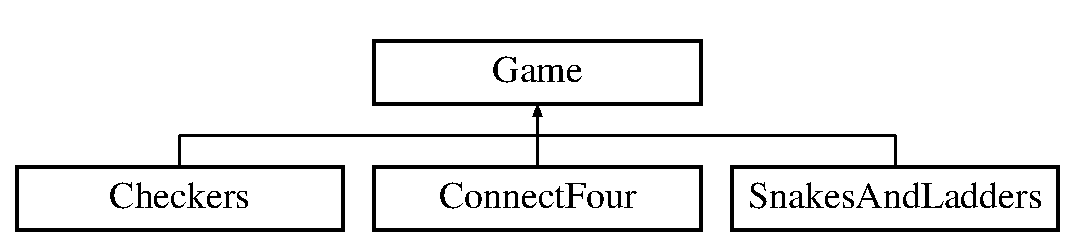
\includegraphics[height=2.000000cm]{classGame}
\end{center}
\end{figure}
\subsection*{Public Member Functions}
\begin{DoxyCompactItemize}
\item 
\hyperlink{classGame_ad2ad634188c8b6151d74cbcc4f858d81}{Game} (const int \hyperlink{classGame_a2a64a5ac5fe7466f02392d7bc75cf372}{amount\-Of\-Players}, const int \hyperlink{classGame_a33dcee5dd512148a0b12aa7fba41b5da}{columns}, const int \hyperlink{classGame_ae882486dec6d9507bbef7f44aaf07db5}{rows})
\item 
virtual void \hyperlink{classGame_a3d9b98f7c4a96ecf578f75b96c9f0e90}{start} ()
\item 
virtual \hyperlink{classGame_ae3d112ca6e0e55150d2fdbc704474530}{$\sim$\-Game} ()
\end{DoxyCompactItemize}
\subsection*{Protected Member Functions}
\begin{DoxyCompactItemize}
\item 
void \hyperlink{classGame_a43a51eaa8b6fdb3dc6faa4d3417bad1e}{clear\-Screen} ()
\begin{DoxyCompactList}\small\item\em Clears the terminal window. \end{DoxyCompactList}\item 
virtual void \hyperlink{classGame_a7034c849d9fb62c74edb0a43f66b3bba}{draw\-Screen} ()=0
\begin{DoxyCompactList}\small\item\em Draws out the board as required. \end{DoxyCompactList}\item 
virtual bool \hyperlink{classGame_a4986ef96dee8f573ba1532dfe3ee8a4a}{get\-Move} ()=0
\begin{DoxyCompactList}\small\item\em Gets input from the player detailing which move they wish to make. \end{DoxyCompactList}\item 
virtual int \hyperlink{classGame_ada584c598be0f7066a396e1677ad7dc6}{is\-Over} ()=0
\begin{DoxyCompactList}\small\item\em Defines whether or not the game is over. \end{DoxyCompactList}\end{DoxyCompactItemize}
\subsection*{Protected Attributes}
\begin{DoxyCompactItemize}
\item 
const int \hyperlink{classGame_a2a64a5ac5fe7466f02392d7bc75cf372}{amount\-Of\-Players}
\begin{DoxyCompactList}\small\item\em Holds the length of the players array. \end{DoxyCompactList}\item 
const int \hyperlink{classGame_a33dcee5dd512148a0b12aa7fba41b5da}{columns}
\begin{DoxyCompactList}\small\item\em Holds the amount of columns within the grid. \end{DoxyCompactList}\item 
int \hyperlink{classGame_af57daa2f1aef9f264c18b462f8294e52}{current\-Player}
\begin{DoxyCompactList}\small\item\em Holds the position in the players array of the current player. \end{DoxyCompactList}\item 
\hyperlink{classSquare}{Square} $\ast$$\ast$ \hyperlink{classGame_a44fda9d5235865323c59d95b1f59b459}{grid}
\begin{DoxyCompactList}\small\item\em Holds all of the squares that makes up the games grid. \end{DoxyCompactList}\item 
\hyperlink{classPlayer}{Player} $\ast$$\ast$ \hyperlink{classGame_ad82f617ca44c8996333c7f41c410a56b}{players}
\begin{DoxyCompactList}\small\item\em Holds all of the games players. \end{DoxyCompactList}\item 
const int \hyperlink{classGame_ae882486dec6d9507bbef7f44aaf07db5}{rows}
\begin{DoxyCompactList}\small\item\em Holds the amount of rows within the grid. \end{DoxyCompactList}\end{DoxyCompactItemize}


\subsection{Detailed Description}
Base foundation for all of the games. \begin{DoxyAuthor}{Author}
Ian Duffy 

Darren Brogan 
\end{DoxyAuthor}


Definition at line 19 of file Game.\-h.



\subsection{Constructor \& Destructor Documentation}
\hypertarget{classGame_ad2ad634188c8b6151d74cbcc4f858d81}{\index{Game@{Game}!Game@{Game}}
\index{Game@{Game}!Game@{Game}}
\subsubsection[{Game}]{\setlength{\rightskip}{0pt plus 5cm}Game\-::\-Game (
\begin{DoxyParamCaption}
\item[{const int}]{amount\-Of\-Players, }
\item[{const int}]{columns, }
\item[{const int}]{rows}
\end{DoxyParamCaption}
)}}\label{classGame_ad2ad634188c8b6151d74cbcc4f858d81}


Definition at line 10 of file Game.\-cpp.

\hypertarget{classGame_ae3d112ca6e0e55150d2fdbc704474530}{\index{Game@{Game}!$\sim$\-Game@{$\sim$\-Game}}
\index{$\sim$\-Game@{$\sim$\-Game}!Game@{Game}}
\subsubsection[{$\sim$\-Game}]{\setlength{\rightskip}{0pt plus 5cm}Game\-::$\sim$\-Game (
\begin{DoxyParamCaption}
{}
\end{DoxyParamCaption}
)\hspace{0.3cm}{\ttfamily [virtual]}}}\label{classGame_ae3d112ca6e0e55150d2fdbc704474530}


Definition at line 20 of file Game.\-cpp.



\subsection{Member Function Documentation}
\hypertarget{classGame_a43a51eaa8b6fdb3dc6faa4d3417bad1e}{\index{Game@{Game}!clear\-Screen@{clear\-Screen}}
\index{clear\-Screen@{clear\-Screen}!Game@{Game}}
\subsubsection[{clear\-Screen}]{\setlength{\rightskip}{0pt plus 5cm}void Game\-::clear\-Screen (
\begin{DoxyParamCaption}
{}
\end{DoxyParamCaption}
)\hspace{0.3cm}{\ttfamily [protected]}}}\label{classGame_a43a51eaa8b6fdb3dc6faa4d3417bad1e}


Clears the terminal window. 



Definition at line 49 of file Game.\-cpp.

\hypertarget{classGame_a7034c849d9fb62c74edb0a43f66b3bba}{\index{Game@{Game}!draw\-Screen@{draw\-Screen}}
\index{draw\-Screen@{draw\-Screen}!Game@{Game}}
\subsubsection[{draw\-Screen}]{\setlength{\rightskip}{0pt plus 5cm}virtual void Game\-::draw\-Screen (
\begin{DoxyParamCaption}
{}
\end{DoxyParamCaption}
)\hspace{0.3cm}{\ttfamily [protected]}, {\ttfamily [pure virtual]}}}\label{classGame_a7034c849d9fb62c74edb0a43f66b3bba}


Draws out the board as required. 

\hypertarget{classGame_a4986ef96dee8f573ba1532dfe3ee8a4a}{\index{Game@{Game}!get\-Move@{get\-Move}}
\index{get\-Move@{get\-Move}!Game@{Game}}
\subsubsection[{get\-Move}]{\setlength{\rightskip}{0pt plus 5cm}virtual bool Game\-::get\-Move (
\begin{DoxyParamCaption}
{}
\end{DoxyParamCaption}
)\hspace{0.3cm}{\ttfamily [protected]}, {\ttfamily [pure virtual]}}}\label{classGame_a4986ef96dee8f573ba1532dfe3ee8a4a}


Gets input from the player detailing which move they wish to make. 

\hypertarget{classGame_ada584c598be0f7066a396e1677ad7dc6}{\index{Game@{Game}!is\-Over@{is\-Over}}
\index{is\-Over@{is\-Over}!Game@{Game}}
\subsubsection[{is\-Over}]{\setlength{\rightskip}{0pt plus 5cm}virtual int Game\-::is\-Over (
\begin{DoxyParamCaption}
{}
\end{DoxyParamCaption}
)\hspace{0.3cm}{\ttfamily [protected]}, {\ttfamily [pure virtual]}}}\label{classGame_ada584c598be0f7066a396e1677ad7dc6}


Defines whether or not the game is over. 

\hypertarget{classGame_a3d9b98f7c4a96ecf578f75b96c9f0e90}{\index{Game@{Game}!start@{start}}
\index{start@{start}!Game@{Game}}
\subsubsection[{start}]{\setlength{\rightskip}{0pt plus 5cm}void Game\-::start (
\begin{DoxyParamCaption}
{}
\end{DoxyParamCaption}
)\hspace{0.3cm}{\ttfamily [virtual]}}}\label{classGame_a3d9b98f7c4a96ecf578f75b96c9f0e90}
Controls the flow of the game, Continues to call \hyperlink{classGame_a4986ef96dee8f573ba1532dfe3ee8a4a}{get\-Move()} until \hyperlink{classGame_ada584c598be0f7066a396e1677ad7dc6}{is\-Over()} returns something other than 0. 

Definition at line 30 of file Game.\-cpp.



\subsection{Field Documentation}
\hypertarget{classGame_a2a64a5ac5fe7466f02392d7bc75cf372}{\index{Game@{Game}!amount\-Of\-Players@{amount\-Of\-Players}}
\index{amount\-Of\-Players@{amount\-Of\-Players}!Game@{Game}}
\subsubsection[{amount\-Of\-Players}]{\setlength{\rightskip}{0pt plus 5cm}const int Game\-::amount\-Of\-Players\hspace{0.3cm}{\ttfamily [protected]}}}\label{classGame_a2a64a5ac5fe7466f02392d7bc75cf372}


Holds the length of the players array. 



Definition at line 31 of file Game.\-h.

\hypertarget{classGame_a33dcee5dd512148a0b12aa7fba41b5da}{\index{Game@{Game}!columns@{columns}}
\index{columns@{columns}!Game@{Game}}
\subsubsection[{columns}]{\setlength{\rightskip}{0pt plus 5cm}const int Game\-::columns\hspace{0.3cm}{\ttfamily [protected]}}}\label{classGame_a33dcee5dd512148a0b12aa7fba41b5da}


Holds the amount of columns within the grid. 



Definition at line 34 of file Game.\-h.

\hypertarget{classGame_af57daa2f1aef9f264c18b462f8294e52}{\index{Game@{Game}!current\-Player@{current\-Player}}
\index{current\-Player@{current\-Player}!Game@{Game}}
\subsubsection[{current\-Player}]{\setlength{\rightskip}{0pt plus 5cm}int Game\-::current\-Player\hspace{0.3cm}{\ttfamily [protected]}}}\label{classGame_af57daa2f1aef9f264c18b462f8294e52}


Holds the position in the players array of the current player. 



Definition at line 22 of file Game.\-h.

\hypertarget{classGame_a44fda9d5235865323c59d95b1f59b459}{\index{Game@{Game}!grid@{grid}}
\index{grid@{grid}!Game@{Game}}
\subsubsection[{grid}]{\setlength{\rightskip}{0pt plus 5cm}{\bf Square}$\ast$$\ast$ Game\-::grid\hspace{0.3cm}{\ttfamily [protected]}}}\label{classGame_a44fda9d5235865323c59d95b1f59b459}


Holds all of the squares that makes up the games grid. 



Definition at line 28 of file Game.\-h.

\hypertarget{classGame_ad82f617ca44c8996333c7f41c410a56b}{\index{Game@{Game}!players@{players}}
\index{players@{players}!Game@{Game}}
\subsubsection[{players}]{\setlength{\rightskip}{0pt plus 5cm}{\bf Player}$\ast$$\ast$ Game\-::players\hspace{0.3cm}{\ttfamily [protected]}}}\label{classGame_ad82f617ca44c8996333c7f41c410a56b}


Holds all of the games players. 



Definition at line 25 of file Game.\-h.

\hypertarget{classGame_ae882486dec6d9507bbef7f44aaf07db5}{\index{Game@{Game}!rows@{rows}}
\index{rows@{rows}!Game@{Game}}
\subsubsection[{rows}]{\setlength{\rightskip}{0pt plus 5cm}const int Game\-::rows\hspace{0.3cm}{\ttfamily [protected]}}}\label{classGame_ae882486dec6d9507bbef7f44aaf07db5}


Holds the amount of rows within the grid. 



Definition at line 37 of file Game.\-h.



The documentation for this class was generated from the following files\-:\begin{DoxyCompactItemize}
\item 
\hyperlink{Game_8h}{Game.\-h}\item 
\hyperlink{Game_8cpp}{Game.\-cpp}\end{DoxyCompactItemize}

\hypertarget{classIdentifierPiece}{\section{Identifier\-Piece Class Reference}
\label{classIdentifierPiece}\index{Identifier\-Piece@{Identifier\-Piece}}
}


{\ttfamily \#include $<$Identifier\-Piece.\-h$>$}

Inheritance diagram for Identifier\-Piece\-:\begin{figure}[H]
\begin{center}
\leavevmode
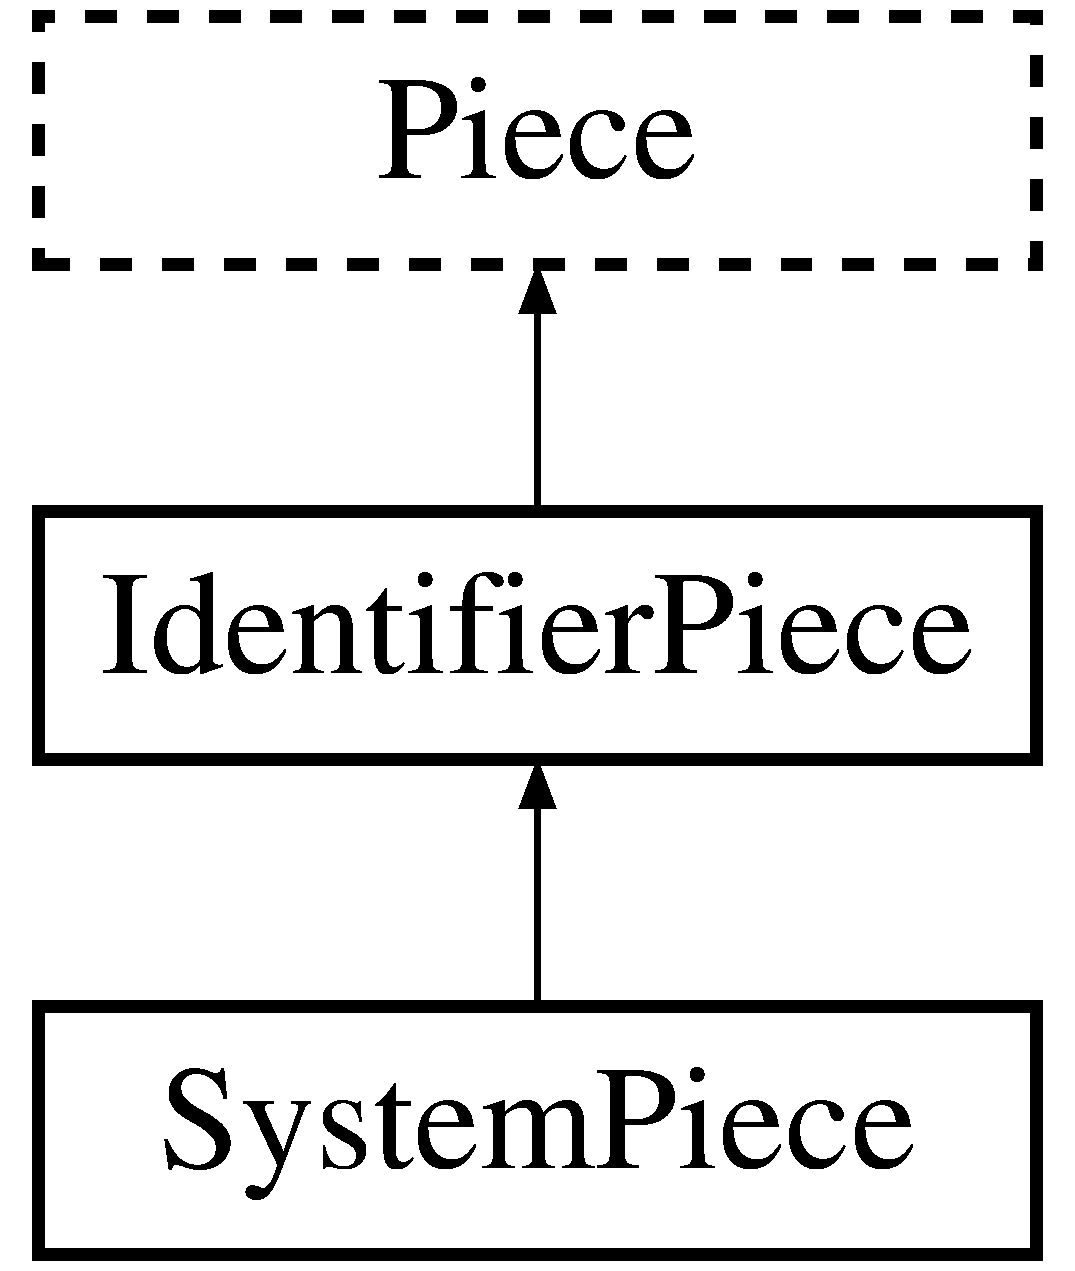
\includegraphics[height=3.000000cm]{classIdentifierPiece}
\end{center}
\end{figure}
\subsection*{Public Member Functions}
\begin{DoxyCompactItemize}
\item 
int \hyperlink{classIdentifierPiece_aee7fb7f81fa27380620bf10294487b42}{get\-Identifier} ()
\begin{DoxyCompactList}\small\item\em Returns the identifier. \end{DoxyCompactList}\item 
\hyperlink{classIdentifierPiece_a88d7eedf40b3507a0bad13fd7179b87d}{Identifier\-Piece} (\hyperlink{classPlayer}{Player} $\ast$\hyperlink{classPiece_a43beac3b5268343b9f7e575d637eda98}{owner}, int \hyperlink{classIdentifierPiece_aab84613c911d8d7c269b9636ce6faa36}{identifier})
\item 
virtual void \hyperlink{classIdentifierPiece_a63030a6e3daf72f81d2731e809e30d5b}{print} (ostream \&os) const 
\begin{DoxyCompactList}\small\item\em Override the print function to include the identifier. \end{DoxyCompactList}\end{DoxyCompactItemize}
\subsection*{Protected Attributes}
\begin{DoxyCompactItemize}
\item 
int \hyperlink{classIdentifierPiece_aab84613c911d8d7c269b9636ce6faa36}{identifier}
\begin{DoxyCompactList}\small\item\em The piece's identifier. \end{DoxyCompactList}\end{DoxyCompactItemize}
\subsection*{Additional Inherited Members}


\subsection{Detailed Description}
A \hyperlink{classPiece}{Piece} with an identifier. \begin{DoxyAuthor}{Author}
Ian Duffy. 
\end{DoxyAuthor}


Definition at line 9 of file Identifier\-Piece.\-h.



\subsection{Constructor \& Destructor Documentation}
\hypertarget{classIdentifierPiece_a88d7eedf40b3507a0bad13fd7179b87d}{\index{Identifier\-Piece@{Identifier\-Piece}!Identifier\-Piece@{Identifier\-Piece}}
\index{Identifier\-Piece@{Identifier\-Piece}!IdentifierPiece@{Identifier\-Piece}}
\subsubsection[{Identifier\-Piece}]{\setlength{\rightskip}{0pt plus 5cm}Identifier\-Piece\-::\-Identifier\-Piece (
\begin{DoxyParamCaption}
\item[{{\bf Player} $\ast$}]{owner, }
\item[{int}]{identifier}
\end{DoxyParamCaption}
)}}\label{classIdentifierPiece_a88d7eedf40b3507a0bad13fd7179b87d}
A \hyperlink{classPiece}{Piece} with an identifier. \begin{DoxyAuthor}{Author}
Ian Duffy. 
\end{DoxyAuthor}


Definition at line 6 of file Identifier\-Piece.\-cpp.



\subsection{Member Function Documentation}
\hypertarget{classIdentifierPiece_aee7fb7f81fa27380620bf10294487b42}{\index{Identifier\-Piece@{Identifier\-Piece}!get\-Identifier@{get\-Identifier}}
\index{get\-Identifier@{get\-Identifier}!IdentifierPiece@{Identifier\-Piece}}
\subsubsection[{get\-Identifier}]{\setlength{\rightskip}{0pt plus 5cm}int Identifier\-Piece\-::get\-Identifier (
\begin{DoxyParamCaption}
{}
\end{DoxyParamCaption}
)}}\label{classIdentifierPiece_aee7fb7f81fa27380620bf10294487b42}


Returns the identifier. 



Definition at line 18 of file Identifier\-Piece.\-cpp.

\hypertarget{classIdentifierPiece_a63030a6e3daf72f81d2731e809e30d5b}{\index{Identifier\-Piece@{Identifier\-Piece}!print@{print}}
\index{print@{print}!IdentifierPiece@{Identifier\-Piece}}
\subsubsection[{print}]{\setlength{\rightskip}{0pt plus 5cm}void Identifier\-Piece\-::print (
\begin{DoxyParamCaption}
\item[{ostream \&}]{os}
\end{DoxyParamCaption}
) const\hspace{0.3cm}{\ttfamily [virtual]}}}\label{classIdentifierPiece_a63030a6e3daf72f81d2731e809e30d5b}


Override the print function to include the identifier. 



Reimplemented from \hyperlink{classPiece_aace14e1a78a22394f997b045fe31e84a}{Piece}.



Definition at line 12 of file Identifier\-Piece.\-cpp.



\subsection{Field Documentation}
\hypertarget{classIdentifierPiece_aab84613c911d8d7c269b9636ce6faa36}{\index{Identifier\-Piece@{Identifier\-Piece}!identifier@{identifier}}
\index{identifier@{identifier}!IdentifierPiece@{Identifier\-Piece}}
\subsubsection[{identifier}]{\setlength{\rightskip}{0pt plus 5cm}int Identifier\-Piece\-::identifier\hspace{0.3cm}{\ttfamily [protected]}}}\label{classIdentifierPiece_aab84613c911d8d7c269b9636ce6faa36}


The piece's identifier. 



Definition at line 12 of file Identifier\-Piece.\-h.



The documentation for this class was generated from the following files\-:\begin{DoxyCompactItemize}
\item 
\hyperlink{IdentifierPiece_8h}{Identifier\-Piece.\-h}\item 
\hyperlink{IdentifierPiece_8cpp}{Identifier\-Piece.\-cpp}\end{DoxyCompactItemize}

\hypertarget{classPiece}{\section{Piece Class Reference}
\label{classPiece}\index{Piece@{Piece}}
}


{\ttfamily \#include $<$Piece.\-h$>$}

Inheritance diagram for Piece\-:\begin{figure}[H]
\begin{center}
\leavevmode
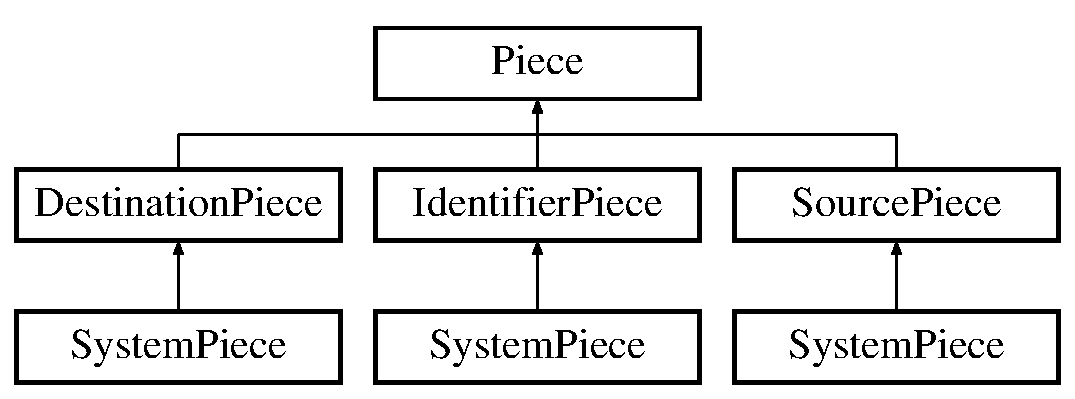
\includegraphics[height=3.000000cm]{classPiece}
\end{center}
\end{figure}
\subsection*{Public Member Functions}
\begin{DoxyCompactItemize}
\item 
int \hyperlink{classPiece_aeebab4a49f40fde49a9698c19f51f4a0}{get\-Type} ()
\begin{DoxyCompactList}\small\item\em Returns the type of piece. \end{DoxyCompactList}\item 
\hyperlink{classPiece_ac57de5803bbad829b143bc7268267dc1}{Piece} ()
\item 
\hyperlink{classPiece_a645709ec114f364073ee432d102b0551}{Piece} (\hyperlink{classPlayer}{Player} $\ast$\hyperlink{classPiece_a43beac3b5268343b9f7e575d637eda98}{owner})
\item 
\hyperlink{classPiece_a72c6f3a5df2036c7743bd91e2daeb5bc}{Piece} (\hyperlink{classPlayer}{Player} $\ast$\hyperlink{classPiece_a43beac3b5268343b9f7e575d637eda98}{owner}, int \hyperlink{classPiece_a5c3c79a15de7daa1efde1b8aa246e8d4}{type})
\item 
virtual void \hyperlink{classPiece_aace14e1a78a22394f997b045fe31e84a}{print} (ostream \&os) const 
\begin{DoxyCompactList}\small\item\em Inserts the piece into the given ostream. \end{DoxyCompactList}\item 
bool \hyperlink{classPiece_acdc19e123cac0d8999ce70953de61aa3}{set\-Type} (int \hyperlink{classPiece_a5c3c79a15de7daa1efde1b8aa246e8d4}{type})
\begin{DoxyCompactList}\small\item\em Sets the type of piece. \end{DoxyCompactList}\item 
virtual \hyperlink{classPiece_a5d7a4f6bade94cb33b6f634de8aa7918}{$\sim$\-Piece} ()
\end{DoxyCompactItemize}
\subsection*{Data Fields}
\begin{DoxyCompactItemize}
\item 
\hyperlink{classPlayer}{Player} $\ast$ \hyperlink{classPiece_a43beac3b5268343b9f7e575d637eda98}{owner}
\begin{DoxyCompactList}\small\item\em Pointer to the pieces owner. \end{DoxyCompactList}\end{DoxyCompactItemize}
\subsection*{Protected Attributes}
\begin{DoxyCompactItemize}
\item 
int \hyperlink{classPiece_a5c3c79a15de7daa1efde1b8aa246e8d4}{type}
\begin{DoxyCompactList}\small\item\em The type of the piece. \end{DoxyCompactList}\end{DoxyCompactItemize}


\subsection{Detailed Description}


Definition at line 15 of file Piece.\-h.



\subsection{Constructor \& Destructor Documentation}
\hypertarget{classPiece_ac57de5803bbad829b143bc7268267dc1}{\index{Piece@{Piece}!Piece@{Piece}}
\index{Piece@{Piece}!Piece@{Piece}}
\subsubsection[{Piece}]{\setlength{\rightskip}{0pt plus 5cm}Piece\-::\-Piece (
\begin{DoxyParamCaption}
{}
\end{DoxyParamCaption}
)}}\label{classPiece_ac57de5803bbad829b143bc7268267dc1}
\hyperlink{classPiece}{Piece} \begin{DoxyAuthor}{Author}
Ian Duffy 

Darren Brogan 
\end{DoxyAuthor}


Definition at line 9 of file Piece.\-cpp.

\hypertarget{classPiece_a645709ec114f364073ee432d102b0551}{\index{Piece@{Piece}!Piece@{Piece}}
\index{Piece@{Piece}!Piece@{Piece}}
\subsubsection[{Piece}]{\setlength{\rightskip}{0pt plus 5cm}Piece\-::\-Piece (
\begin{DoxyParamCaption}
\item[{{\bf Player} $\ast$}]{owner}
\end{DoxyParamCaption}
)}}\label{classPiece_a645709ec114f364073ee432d102b0551}


Definition at line 13 of file Piece.\-cpp.

\hypertarget{classPiece_a72c6f3a5df2036c7743bd91e2daeb5bc}{\index{Piece@{Piece}!Piece@{Piece}}
\index{Piece@{Piece}!Piece@{Piece}}
\subsubsection[{Piece}]{\setlength{\rightskip}{0pt plus 5cm}Piece\-::\-Piece (
\begin{DoxyParamCaption}
\item[{{\bf Player} $\ast$}]{owner, }
\item[{int}]{type}
\end{DoxyParamCaption}
)}}\label{classPiece_a72c6f3a5df2036c7743bd91e2daeb5bc}
\hypertarget{classPiece_a5d7a4f6bade94cb33b6f634de8aa7918}{\index{Piece@{Piece}!$\sim$\-Piece@{$\sim$\-Piece}}
\index{$\sim$\-Piece@{$\sim$\-Piece}!Piece@{Piece}}
\subsubsection[{$\sim$\-Piece}]{\setlength{\rightskip}{0pt plus 5cm}Piece\-::$\sim$\-Piece (
\begin{DoxyParamCaption}
{}
\end{DoxyParamCaption}
)\hspace{0.3cm}{\ttfamily [virtual]}}}\label{classPiece_a5d7a4f6bade94cb33b6f634de8aa7918}


Definition at line 18 of file Piece.\-cpp.



\subsection{Member Function Documentation}
\hypertarget{classPiece_aeebab4a49f40fde49a9698c19f51f4a0}{\index{Piece@{Piece}!get\-Type@{get\-Type}}
\index{get\-Type@{get\-Type}!Piece@{Piece}}
\subsubsection[{get\-Type}]{\setlength{\rightskip}{0pt plus 5cm}int Piece\-::get\-Type (
\begin{DoxyParamCaption}
{}
\end{DoxyParamCaption}
)}}\label{classPiece_aeebab4a49f40fde49a9698c19f51f4a0}


Returns the type of piece. 



Definition at line 22 of file Piece.\-cpp.

\hypertarget{classPiece_aace14e1a78a22394f997b045fe31e84a}{\index{Piece@{Piece}!print@{print}}
\index{print@{print}!Piece@{Piece}}
\subsubsection[{print}]{\setlength{\rightskip}{0pt plus 5cm}void Piece\-::print (
\begin{DoxyParamCaption}
\item[{ostream \&}]{os}
\end{DoxyParamCaption}
) const\hspace{0.3cm}{\ttfamily [virtual]}}}\label{classPiece_aace14e1a78a22394f997b045fe31e84a}


Inserts the piece into the given ostream. 



Reimplemented in \hyperlink{classIdentifierPiece_a63030a6e3daf72f81d2731e809e30d5b}{Identifier\-Piece}.



Definition at line 37 of file Piece.\-cpp.

\hypertarget{classPiece_acdc19e123cac0d8999ce70953de61aa3}{\index{Piece@{Piece}!set\-Type@{set\-Type}}
\index{set\-Type@{set\-Type}!Piece@{Piece}}
\subsubsection[{set\-Type}]{\setlength{\rightskip}{0pt plus 5cm}bool Piece\-::set\-Type (
\begin{DoxyParamCaption}
\item[{int}]{type}
\end{DoxyParamCaption}
)}}\label{classPiece_acdc19e123cac0d8999ce70953de61aa3}


Sets the type of piece. 



Definition at line 27 of file Piece.\-cpp.



\subsection{Field Documentation}
\hypertarget{classPiece_a43beac3b5268343b9f7e575d637eda98}{\index{Piece@{Piece}!owner@{owner}}
\index{owner@{owner}!Piece@{Piece}}
\subsubsection[{owner}]{\setlength{\rightskip}{0pt plus 5cm}{\bf Player}$\ast$ Piece\-::owner}}\label{classPiece_a43beac3b5268343b9f7e575d637eda98}


Pointer to the pieces owner. 



Definition at line 36 of file Piece.\-h.

\hypertarget{classPiece_a5c3c79a15de7daa1efde1b8aa246e8d4}{\index{Piece@{Piece}!type@{type}}
\index{type@{type}!Piece@{Piece}}
\subsubsection[{type}]{\setlength{\rightskip}{0pt plus 5cm}int Piece\-::type\hspace{0.3cm}{\ttfamily [protected]}}}\label{classPiece_a5c3c79a15de7daa1efde1b8aa246e8d4}


The type of the piece. 



Definition at line 18 of file Piece.\-h.



The documentation for this class was generated from the following files\-:\begin{DoxyCompactItemize}
\item 
\hyperlink{Piece_8h}{Piece.\-h}\item 
\hyperlink{Piece_8cpp}{Piece.\-cpp}\end{DoxyCompactItemize}

\hypertarget{classPlayer}{\section{Player Class Reference}
\label{classPlayer}\index{Player@{Player}}
}


{\ttfamily \#include $<$Player.\-h$>$}

Inheritance diagram for Player\-:\begin{figure}[H]
\begin{center}
\leavevmode
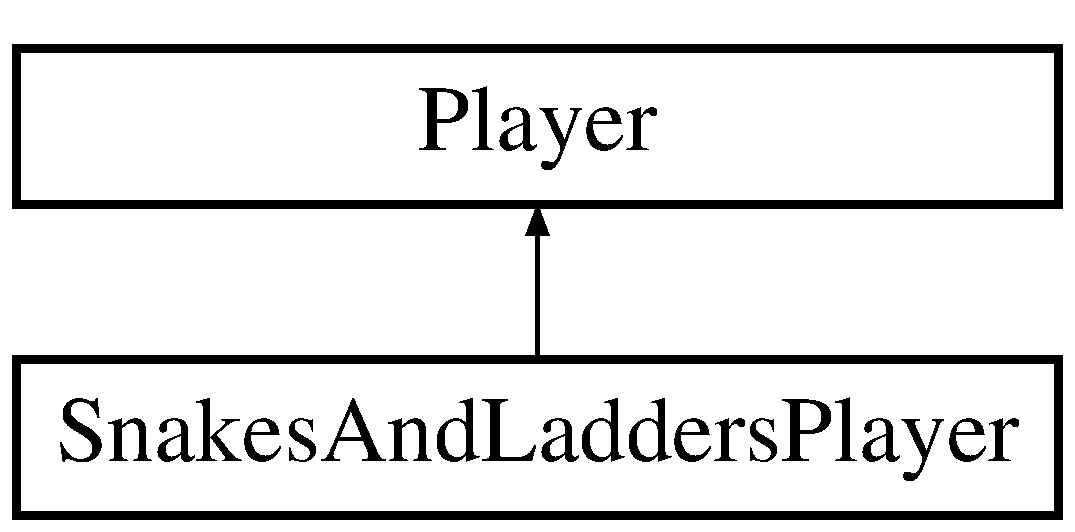
\includegraphics[height=2.000000cm]{classPlayer}
\end{center}
\end{figure}
\subsection*{Public Member Functions}
\begin{DoxyCompactItemize}
\item 
\hyperlink{classPiece}{Piece} $\ast$ \hyperlink{classPlayer_ad09c5fa121693aebd9324f5a67b2a4b4}{add\-Piece} ()
\begin{DoxyCompactList}\small\item\em Add pieces to the pieces vector. \end{DoxyCompactList}\item 
\hyperlink{classPiece}{Piece} $\ast$ \hyperlink{classPlayer_acf6a704d66c88132eff94fe0db15ead7}{add\-Piece} (\hyperlink{classPiece}{Piece} $\ast$insert)
\item 
int \hyperlink{classPlayer_a5a545f24c6c256c126cd73f1f9625060}{get\-Amount\-Of\-Pieces} ()
\begin{DoxyCompactList}\small\item\em Public functions. \end{DoxyCompactList}\item 
string \hyperlink{classPlayer_a17af53ee144ccdd489f1d2a88d23b534}{get\-Character} (int type)
\begin{DoxyCompactList}\small\item\em Returns a string from pieces vector at index type. \end{DoxyCompactList}\item 
\hyperlink{classPiece}{Piece} $\ast$ \hyperlink{classPlayer_a8067bf22b680314eb5767753e76b114c}{get\-Piece} (int index)
\begin{DoxyCompactList}\small\item\em Returns a pointer to the piece in the pieces vector at index index. \end{DoxyCompactList}\item 
bool \hyperlink{classPlayer_af053c37a04f7881f5e76272d8c4fc7e6}{has\-Type} (int type)
\begin{DoxyCompactList}\small\item\em Check if pieces vector at index type is empty. \end{DoxyCompactList}\item 
\hyperlink{classPlayer_affe0cc3cb714f6deb4e62f0c0d3f1fd8}{Player} ()
\begin{DoxyCompactList}\small\item\em Public constructors. \end{DoxyCompactList}\item 
\hyperlink{classPlayer_acc7e5bcd2a68c9f89811140e27ebe09c}{Player} (int \hyperlink{classPlayer_a677f323efe4a7534a054345a4d99d40f}{amount\-Of\-Types}, vector$<$ string $>$ \hyperlink{classPlayer_a05f23ead572f763fedd4488d6a82b822}{types}, int \hyperlink{classPlayer_a69e6c3b3ae77235f6f47c49b09e67331}{max\-Pieces})
\item 
bool \hyperlink{classPlayer_a255abeb598abb76c3fb8b82bc39563a0}{remove\-Piece} ()
\item 
virtual \hyperlink{classPlayer_a749d2c00e1fe0f5c2746f7505a58c062}{$\sim$\-Player} ()
\end{DoxyCompactItemize}
\subsection*{Data Fields}
\begin{DoxyCompactItemize}
\item 
bool \hyperlink{classPlayer_a915c6031e68208b409ce8550419f6247}{suspended}
\begin{DoxyCompactList}\small\item\em Return weather this player can move or not. \end{DoxyCompactList}\end{DoxyCompactItemize}
\subsection*{Protected Attributes}
\begin{DoxyCompactItemize}
\item 
int \hyperlink{classPlayer_a02564dff78d55061c0afa08bfa5342e5}{amount\-Of\-Pieces}
\item 
int \hyperlink{classPlayer_a677f323efe4a7534a054345a4d99d40f}{amount\-Of\-Types}
\begin{DoxyCompactList}\small\item\em Variable used to store the amount of types of pieces the player has. \end{DoxyCompactList}\item 
int \hyperlink{classPlayer_a69e6c3b3ae77235f6f47c49b09e67331}{max\-Pieces}
\begin{DoxyCompactList}\small\item\em Int variable to store the max amount of pieces a player could own. \end{DoxyCompactList}\item 
vector$<$ \hyperlink{classPiece}{Piece} $\ast$ $>$ \hyperlink{classPlayer_a4e28d717089267557d014e440e910a3b}{pieces}
\begin{DoxyCompactList}\small\item\em Vector of type \hyperlink{classPiece}{Piece} pointer to store all the pieces the player owns. \end{DoxyCompactList}\item 
vector$<$ string $>$ \hyperlink{classPlayer_a05f23ead572f763fedd4488d6a82b822}{types}
\begin{DoxyCompactList}\small\item\em Vector to store the different types of pieces the player could own. \end{DoxyCompactList}\end{DoxyCompactItemize}


\subsection{Detailed Description}


Definition at line 12 of file Player.\-h.



\subsection{Constructor \& Destructor Documentation}
\hypertarget{classPlayer_affe0cc3cb714f6deb4e62f0c0d3f1fd8}{\index{Player@{Player}!Player@{Player}}
\index{Player@{Player}!Player@{Player}}
\subsubsection[{Player}]{\setlength{\rightskip}{0pt plus 5cm}Player\-::\-Player (
\begin{DoxyParamCaption}
{}
\end{DoxyParamCaption}
)}}\label{classPlayer_affe0cc3cb714f6deb4e62f0c0d3f1fd8}


Public constructors. 



Definition at line 4 of file Player.\-cpp.

\hypertarget{classPlayer_acc7e5bcd2a68c9f89811140e27ebe09c}{\index{Player@{Player}!Player@{Player}}
\index{Player@{Player}!Player@{Player}}
\subsubsection[{Player}]{\setlength{\rightskip}{0pt plus 5cm}Player\-::\-Player (
\begin{DoxyParamCaption}
\item[{int}]{amount\-Of\-Types, }
\item[{vector$<$ string $>$}]{types, }
\item[{int}]{max\-Pieces}
\end{DoxyParamCaption}
)}}\label{classPlayer_acc7e5bcd2a68c9f89811140e27ebe09c}


Definition at line 6 of file Player.\-cpp.

\hypertarget{classPlayer_a749d2c00e1fe0f5c2746f7505a58c062}{\index{Player@{Player}!$\sim$\-Player@{$\sim$\-Player}}
\index{$\sim$\-Player@{$\sim$\-Player}!Player@{Player}}
\subsubsection[{$\sim$\-Player}]{\setlength{\rightskip}{0pt plus 5cm}Player\-::$\sim$\-Player (
\begin{DoxyParamCaption}
{}
\end{DoxyParamCaption}
)\hspace{0.3cm}{\ttfamily [virtual]}}}\label{classPlayer_a749d2c00e1fe0f5c2746f7505a58c062}


Definition at line 70 of file Player.\-cpp.



\subsection{Member Function Documentation}
\hypertarget{classPlayer_ad09c5fa121693aebd9324f5a67b2a4b4}{\index{Player@{Player}!add\-Piece@{add\-Piece}}
\index{add\-Piece@{add\-Piece}!Player@{Player}}
\subsubsection[{add\-Piece}]{\setlength{\rightskip}{0pt plus 5cm}{\bf Piece} $\ast$ Player\-::add\-Piece (
\begin{DoxyParamCaption}
{}
\end{DoxyParamCaption}
)}}\label{classPlayer_ad09c5fa121693aebd9324f5a67b2a4b4}


Add pieces to the pieces vector. 



Definition at line 28 of file Player.\-cpp.

\hypertarget{classPlayer_acf6a704d66c88132eff94fe0db15ead7}{\index{Player@{Player}!add\-Piece@{add\-Piece}}
\index{add\-Piece@{add\-Piece}!Player@{Player}}
\subsubsection[{add\-Piece}]{\setlength{\rightskip}{0pt plus 5cm}{\bf Piece} $\ast$ Player\-::add\-Piece (
\begin{DoxyParamCaption}
\item[{{\bf Piece} $\ast$}]{insert}
\end{DoxyParamCaption}
)}}\label{classPlayer_acf6a704d66c88132eff94fe0db15ead7}


Definition at line 39 of file Player.\-cpp.

\hypertarget{classPlayer_a5a545f24c6c256c126cd73f1f9625060}{\index{Player@{Player}!get\-Amount\-Of\-Pieces@{get\-Amount\-Of\-Pieces}}
\index{get\-Amount\-Of\-Pieces@{get\-Amount\-Of\-Pieces}!Player@{Player}}
\subsubsection[{get\-Amount\-Of\-Pieces}]{\setlength{\rightskip}{0pt plus 5cm}int Player\-::get\-Amount\-Of\-Pieces (
\begin{DoxyParamCaption}
{}
\end{DoxyParamCaption}
)}}\label{classPlayer_a5a545f24c6c256c126cd73f1f9625060}


Public functions. 



Definition at line 58 of file Player.\-cpp.

\hypertarget{classPlayer_a17af53ee144ccdd489f1d2a88d23b534}{\index{Player@{Player}!get\-Character@{get\-Character}}
\index{get\-Character@{get\-Character}!Player@{Player}}
\subsubsection[{get\-Character}]{\setlength{\rightskip}{0pt plus 5cm}std\-::string Player\-::get\-Character (
\begin{DoxyParamCaption}
\item[{int}]{type}
\end{DoxyParamCaption}
)}}\label{classPlayer_a17af53ee144ccdd489f1d2a88d23b534}


Returns a string from pieces vector at index type. 



Definition at line 16 of file Player.\-cpp.

\hypertarget{classPlayer_a8067bf22b680314eb5767753e76b114c}{\index{Player@{Player}!get\-Piece@{get\-Piece}}
\index{get\-Piece@{get\-Piece}!Player@{Player}}
\subsubsection[{get\-Piece}]{\setlength{\rightskip}{0pt plus 5cm}{\bf Piece} $\ast$ Player\-::get\-Piece (
\begin{DoxyParamCaption}
\item[{int}]{index}
\end{DoxyParamCaption}
)}}\label{classPlayer_a8067bf22b680314eb5767753e76b114c}


Returns a pointer to the piece in the pieces vector at index index. 



Definition at line 62 of file Player.\-cpp.

\hypertarget{classPlayer_af053c37a04f7881f5e76272d8c4fc7e6}{\index{Player@{Player}!has\-Type@{has\-Type}}
\index{has\-Type@{has\-Type}!Player@{Player}}
\subsubsection[{has\-Type}]{\setlength{\rightskip}{0pt plus 5cm}bool Player\-::has\-Type (
\begin{DoxyParamCaption}
\item[{int}]{type}
\end{DoxyParamCaption}
)}}\label{classPlayer_af053c37a04f7881f5e76272d8c4fc7e6}


Check if pieces vector at index type is empty. 



Definition at line 20 of file Player.\-cpp.

\hypertarget{classPlayer_a255abeb598abb76c3fb8b82bc39563a0}{\index{Player@{Player}!remove\-Piece@{remove\-Piece}}
\index{remove\-Piece@{remove\-Piece}!Player@{Player}}
\subsubsection[{remove\-Piece}]{\setlength{\rightskip}{0pt plus 5cm}bool Player\-::remove\-Piece (
\begin{DoxyParamCaption}
{}
\end{DoxyParamCaption}
)}}\label{classPlayer_a255abeb598abb76c3fb8b82bc39563a0}
Remove \hyperlink{classPiece}{Piece} from the player and return a bollean to identify if it succeded or failed. 

Definition at line 49 of file Player.\-cpp.



\subsection{Field Documentation}
\hypertarget{classPlayer_a02564dff78d55061c0afa08bfa5342e5}{\index{Player@{Player}!amount\-Of\-Pieces@{amount\-Of\-Pieces}}
\index{amount\-Of\-Pieces@{amount\-Of\-Pieces}!Player@{Player}}
\subsubsection[{amount\-Of\-Pieces}]{\setlength{\rightskip}{0pt plus 5cm}int Player\-::amount\-Of\-Pieces\hspace{0.3cm}{\ttfamily [protected]}}}\label{classPlayer_a02564dff78d55061c0afa08bfa5342e5}
Protected Data. Int to store the amount of pieces the player currently owns. 

Definition at line 16 of file Player.\-h.

\hypertarget{classPlayer_a677f323efe4a7534a054345a4d99d40f}{\index{Player@{Player}!amount\-Of\-Types@{amount\-Of\-Types}}
\index{amount\-Of\-Types@{amount\-Of\-Types}!Player@{Player}}
\subsubsection[{amount\-Of\-Types}]{\setlength{\rightskip}{0pt plus 5cm}int Player\-::amount\-Of\-Types\hspace{0.3cm}{\ttfamily [protected]}}}\label{classPlayer_a677f323efe4a7534a054345a4d99d40f}


Variable used to store the amount of types of pieces the player has. 



Definition at line 22 of file Player.\-h.

\hypertarget{classPlayer_a69e6c3b3ae77235f6f47c49b09e67331}{\index{Player@{Player}!max\-Pieces@{max\-Pieces}}
\index{max\-Pieces@{max\-Pieces}!Player@{Player}}
\subsubsection[{max\-Pieces}]{\setlength{\rightskip}{0pt plus 5cm}int Player\-::max\-Pieces\hspace{0.3cm}{\ttfamily [protected]}}}\label{classPlayer_a69e6c3b3ae77235f6f47c49b09e67331}


Int variable to store the max amount of pieces a player could own. 



Definition at line 19 of file Player.\-h.

\hypertarget{classPlayer_a4e28d717089267557d014e440e910a3b}{\index{Player@{Player}!pieces@{pieces}}
\index{pieces@{pieces}!Player@{Player}}
\subsubsection[{pieces}]{\setlength{\rightskip}{0pt plus 5cm}vector$<${\bf Piece}$\ast$$>$ Player\-::pieces\hspace{0.3cm}{\ttfamily [protected]}}}\label{classPlayer_a4e28d717089267557d014e440e910a3b}


Vector of type \hyperlink{classPiece}{Piece} pointer to store all the pieces the player owns. 



Definition at line 28 of file Player.\-h.

\hypertarget{classPlayer_a915c6031e68208b409ce8550419f6247}{\index{Player@{Player}!suspended@{suspended}}
\index{suspended@{suspended}!Player@{Player}}
\subsubsection[{suspended}]{\setlength{\rightskip}{0pt plus 5cm}bool Player\-::suspended}}\label{classPlayer_a915c6031e68208b409ce8550419f6247}


Return weather this player can move or not. 



Definition at line 57 of file Player.\-h.

\hypertarget{classPlayer_a05f23ead572f763fedd4488d6a82b822}{\index{Player@{Player}!types@{types}}
\index{types@{types}!Player@{Player}}
\subsubsection[{types}]{\setlength{\rightskip}{0pt plus 5cm}vector$<$string$>$ Player\-::types\hspace{0.3cm}{\ttfamily [protected]}}}\label{classPlayer_a05f23ead572f763fedd4488d6a82b822}


Vector to store the different types of pieces the player could own. 



Definition at line 25 of file Player.\-h.



The documentation for this class was generated from the following files\-:\begin{DoxyCompactItemize}
\item 
\hyperlink{Player_8h}{Player.\-h}\item 
\hyperlink{Player_8cpp}{Player.\-cpp}\end{DoxyCompactItemize}

\hypertarget{classSnakesAndLadders}{\section{Snakes\-And\-Ladders Class Reference}
\label{classSnakesAndLadders}\index{Snakes\-And\-Ladders@{Snakes\-And\-Ladders}}
}


{\ttfamily \#include $<$Snakes\-And\-Ladders.\-h$>$}

Inheritance diagram for Snakes\-And\-Ladders\-:\begin{figure}[H]
\begin{center}
\leavevmode
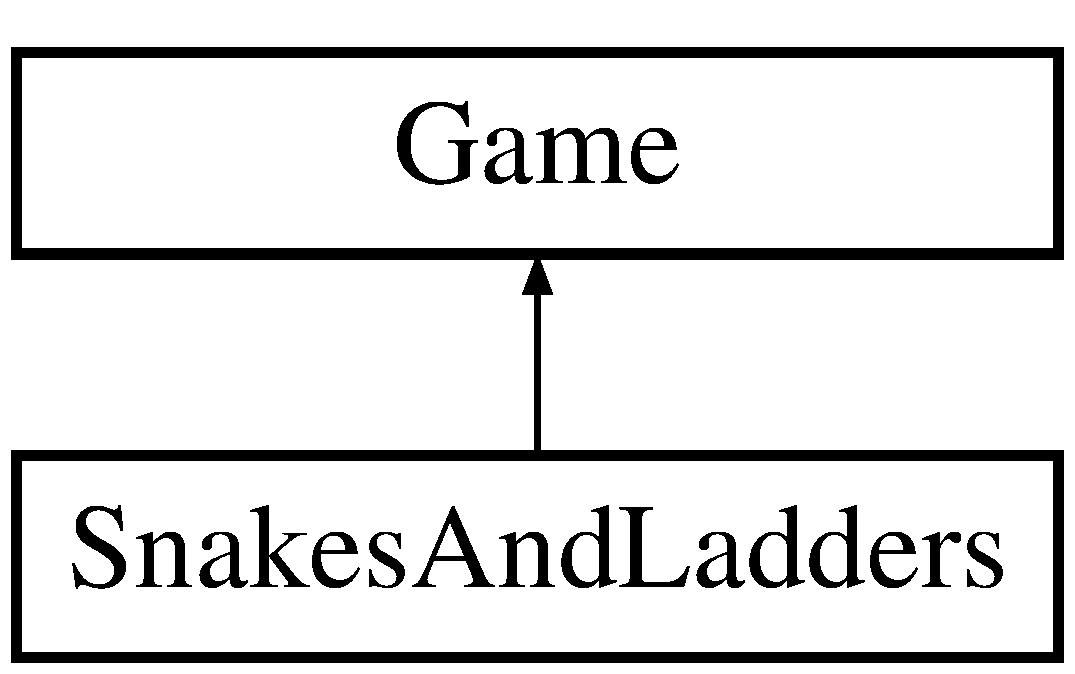
\includegraphics[height=2.000000cm]{classSnakesAndLadders}
\end{center}
\end{figure}
\subsection*{Public Member Functions}
\begin{DoxyCompactItemize}
\item 
\hyperlink{classSnakesAndLadders_ae5de1882a4d4efb8dc62e5a21826f3b6}{Snakes\-And\-Ladders} ()
\item 
\hyperlink{classSnakesAndLadders_a636efaaa9c5ecca3bd580eff1e4e6d5e}{$\sim$\-Snakes\-And\-Ladders} ()
\begin{DoxyCompactList}\small\item\em Deconstructor for snakes and ladders. \end{DoxyCompactList}\end{DoxyCompactItemize}
\subsection*{Additional Inherited Members}


\subsection{Detailed Description}
Snakes and Ladders \hyperlink{classGame}{Game}. \begin{DoxyAuthor}{Author}
Ian Duffy 

Darren Brogan 
\end{DoxyAuthor}


Definition at line 13 of file Snakes\-And\-Ladders.\-h.



\subsection{Constructor \& Destructor Documentation}
\hypertarget{classSnakesAndLadders_ae5de1882a4d4efb8dc62e5a21826f3b6}{\index{Snakes\-And\-Ladders@{Snakes\-And\-Ladders}!Snakes\-And\-Ladders@{Snakes\-And\-Ladders}}
\index{Snakes\-And\-Ladders@{Snakes\-And\-Ladders}!SnakesAndLadders@{Snakes\-And\-Ladders}}
\subsubsection[{Snakes\-And\-Ladders}]{\setlength{\rightskip}{0pt plus 5cm}Snakes\-And\-Ladders\-::\-Snakes\-And\-Ladders (
\begin{DoxyParamCaption}
{}
\end{DoxyParamCaption}
)}}\label{classSnakesAndLadders_ae5de1882a4d4efb8dc62e5a21826f3b6}


Definition at line 15 of file Snakes\-And\-Ladders.\-cpp.

\hypertarget{classSnakesAndLadders_a636efaaa9c5ecca3bd580eff1e4e6d5e}{\index{Snakes\-And\-Ladders@{Snakes\-And\-Ladders}!$\sim$\-Snakes\-And\-Ladders@{$\sim$\-Snakes\-And\-Ladders}}
\index{$\sim$\-Snakes\-And\-Ladders@{$\sim$\-Snakes\-And\-Ladders}!SnakesAndLadders@{Snakes\-And\-Ladders}}
\subsubsection[{$\sim$\-Snakes\-And\-Ladders}]{\setlength{\rightskip}{0pt plus 5cm}Snakes\-And\-Ladders\-::$\sim$\-Snakes\-And\-Ladders (
\begin{DoxyParamCaption}
{}
\end{DoxyParamCaption}
)}}\label{classSnakesAndLadders_a636efaaa9c5ecca3bd580eff1e4e6d5e}


Deconstructor for snakes and ladders. 



Definition at line 136 of file Snakes\-And\-Ladders.\-cpp.



The documentation for this class was generated from the following files\-:\begin{DoxyCompactItemize}
\item 
\hyperlink{SnakesAndLadders_8h}{Snakes\-And\-Ladders.\-h}\item 
\hyperlink{SnakesAndLadders_8cpp}{Snakes\-And\-Ladders.\-cpp}\end{DoxyCompactItemize}

\hypertarget{classSnakesAndLaddersPlayer}{\section{Snakes\-And\-Ladders\-Player Class Reference}
\label{classSnakesAndLaddersPlayer}\index{Snakes\-And\-Ladders\-Player@{Snakes\-And\-Ladders\-Player}}
}


{\ttfamily \#include $<$Snakes\-And\-Ladders\-Player.\-h$>$}

Inheritance diagram for Snakes\-And\-Ladders\-Player\-:\begin{figure}[H]
\begin{center}
\leavevmode
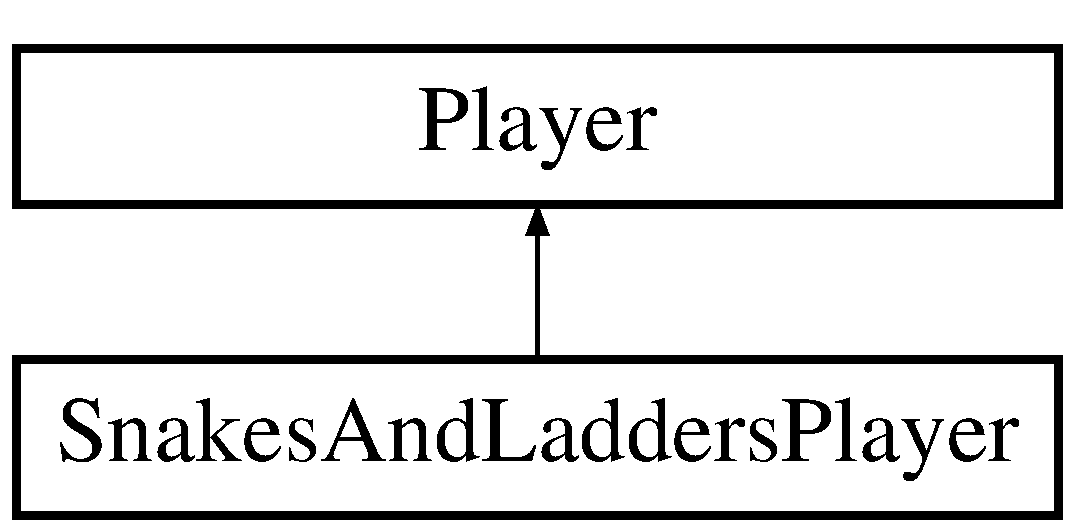
\includegraphics[height=2.000000cm]{classSnakesAndLaddersPlayer}
\end{center}
\end{figure}
\subsection*{Public Member Functions}
\begin{DoxyCompactItemize}
\item 
\hyperlink{classSnakesAndLaddersPlayer_a51b2c254a10ea464cb77915f207995ff}{Snakes\-And\-Ladders\-Player} ()
\item 
\hyperlink{classSnakesAndLaddersPlayer_ae5521be65275b2bc9bc820d757a49c98}{Snakes\-And\-Ladders\-Player} (int \hyperlink{classPlayer_a677f323efe4a7534a054345a4d99d40f}{amount\-Of\-Types}, vector$<$ string $>$ \hyperlink{classPlayer_a05f23ead572f763fedd4488d6a82b822}{types}, int \hyperlink{classPlayer_a69e6c3b3ae77235f6f47c49b09e67331}{max\-Pieces})
\item 
virtual \hyperlink{classSnakesAndLaddersPlayer_a2bdf690e712e815c9a77977a75c4d271}{$\sim$\-Snakes\-And\-Ladders\-Player} ()
\end{DoxyCompactItemize}
\subsection*{Data Fields}
\begin{DoxyCompactItemize}
\item 
bool \hyperlink{classSnakesAndLaddersPlayer_ab6a5f4ff79540545a4f81164cd70e021}{suspended}
\end{DoxyCompactItemize}
\subsection*{Additional Inherited Members}


\subsection{Detailed Description}


Definition at line 6 of file Snakes\-And\-Ladders\-Player.\-h.



\subsection{Constructor \& Destructor Documentation}
\hypertarget{classSnakesAndLaddersPlayer_a51b2c254a10ea464cb77915f207995ff}{\index{Snakes\-And\-Ladders\-Player@{Snakes\-And\-Ladders\-Player}!Snakes\-And\-Ladders\-Player@{Snakes\-And\-Ladders\-Player}}
\index{Snakes\-And\-Ladders\-Player@{Snakes\-And\-Ladders\-Player}!SnakesAndLaddersPlayer@{Snakes\-And\-Ladders\-Player}}
\subsubsection[{Snakes\-And\-Ladders\-Player}]{\setlength{\rightskip}{0pt plus 5cm}Snakes\-And\-Ladders\-Player\-::\-Snakes\-And\-Ladders\-Player (
\begin{DoxyParamCaption}
{}
\end{DoxyParamCaption}
)}}\label{classSnakesAndLaddersPlayer_a51b2c254a10ea464cb77915f207995ff}
\hypertarget{classSnakesAndLaddersPlayer_ae5521be65275b2bc9bc820d757a49c98}{\index{Snakes\-And\-Ladders\-Player@{Snakes\-And\-Ladders\-Player}!Snakes\-And\-Ladders\-Player@{Snakes\-And\-Ladders\-Player}}
\index{Snakes\-And\-Ladders\-Player@{Snakes\-And\-Ladders\-Player}!SnakesAndLaddersPlayer@{Snakes\-And\-Ladders\-Player}}
\subsubsection[{Snakes\-And\-Ladders\-Player}]{\setlength{\rightskip}{0pt plus 5cm}Snakes\-And\-Ladders\-Player\-::\-Snakes\-And\-Ladders\-Player (
\begin{DoxyParamCaption}
\item[{int}]{amount\-Of\-Types, }
\item[{vector$<$ string $>$}]{types, }
\item[{int}]{max\-Pieces}
\end{DoxyParamCaption}
)}}\label{classSnakesAndLaddersPlayer_ae5521be65275b2bc9bc820d757a49c98}


Definition at line 3 of file Snakes\-And\-Ladders\-Player.\-cpp.

\hypertarget{classSnakesAndLaddersPlayer_a2bdf690e712e815c9a77977a75c4d271}{\index{Snakes\-And\-Ladders\-Player@{Snakes\-And\-Ladders\-Player}!$\sim$\-Snakes\-And\-Ladders\-Player@{$\sim$\-Snakes\-And\-Ladders\-Player}}
\index{$\sim$\-Snakes\-And\-Ladders\-Player@{$\sim$\-Snakes\-And\-Ladders\-Player}!SnakesAndLaddersPlayer@{Snakes\-And\-Ladders\-Player}}
\subsubsection[{$\sim$\-Snakes\-And\-Ladders\-Player}]{\setlength{\rightskip}{0pt plus 5cm}Snakes\-And\-Ladders\-Player\-::$\sim$\-Snakes\-And\-Ladders\-Player (
\begin{DoxyParamCaption}
{}
\end{DoxyParamCaption}
)\hspace{0.3cm}{\ttfamily [virtual]}}}\label{classSnakesAndLaddersPlayer_a2bdf690e712e815c9a77977a75c4d271}


Definition at line 9 of file Snakes\-And\-Ladders\-Player.\-cpp.



\subsection{Field Documentation}
\hypertarget{classSnakesAndLaddersPlayer_ab6a5f4ff79540545a4f81164cd70e021}{\index{Snakes\-And\-Ladders\-Player@{Snakes\-And\-Ladders\-Player}!suspended@{suspended}}
\index{suspended@{suspended}!SnakesAndLaddersPlayer@{Snakes\-And\-Ladders\-Player}}
\subsubsection[{suspended}]{\setlength{\rightskip}{0pt plus 5cm}bool Snakes\-And\-Ladders\-Player\-::suspended}}\label{classSnakesAndLaddersPlayer_ab6a5f4ff79540545a4f81164cd70e021}


Definition at line 13 of file Snakes\-And\-Ladders\-Player.\-h.



The documentation for this class was generated from the following files\-:\begin{DoxyCompactItemize}
\item 
\hyperlink{SnakesAndLaddersPlayer_8h}{Snakes\-And\-Ladders\-Player.\-h}\item 
\hyperlink{SnakesAndLaddersPlayer_8cpp}{Snakes\-And\-Ladders\-Player.\-cpp}\end{DoxyCompactItemize}

\hypertarget{classSourcePiece}{\section{Source\-Piece Class Reference}
\label{classSourcePiece}\index{Source\-Piece@{Source\-Piece}}
}


{\ttfamily \#include $<$Source\-Piece.\-h$>$}

Inheritance diagram for Source\-Piece\-:\begin{figure}[H]
\begin{center}
\leavevmode
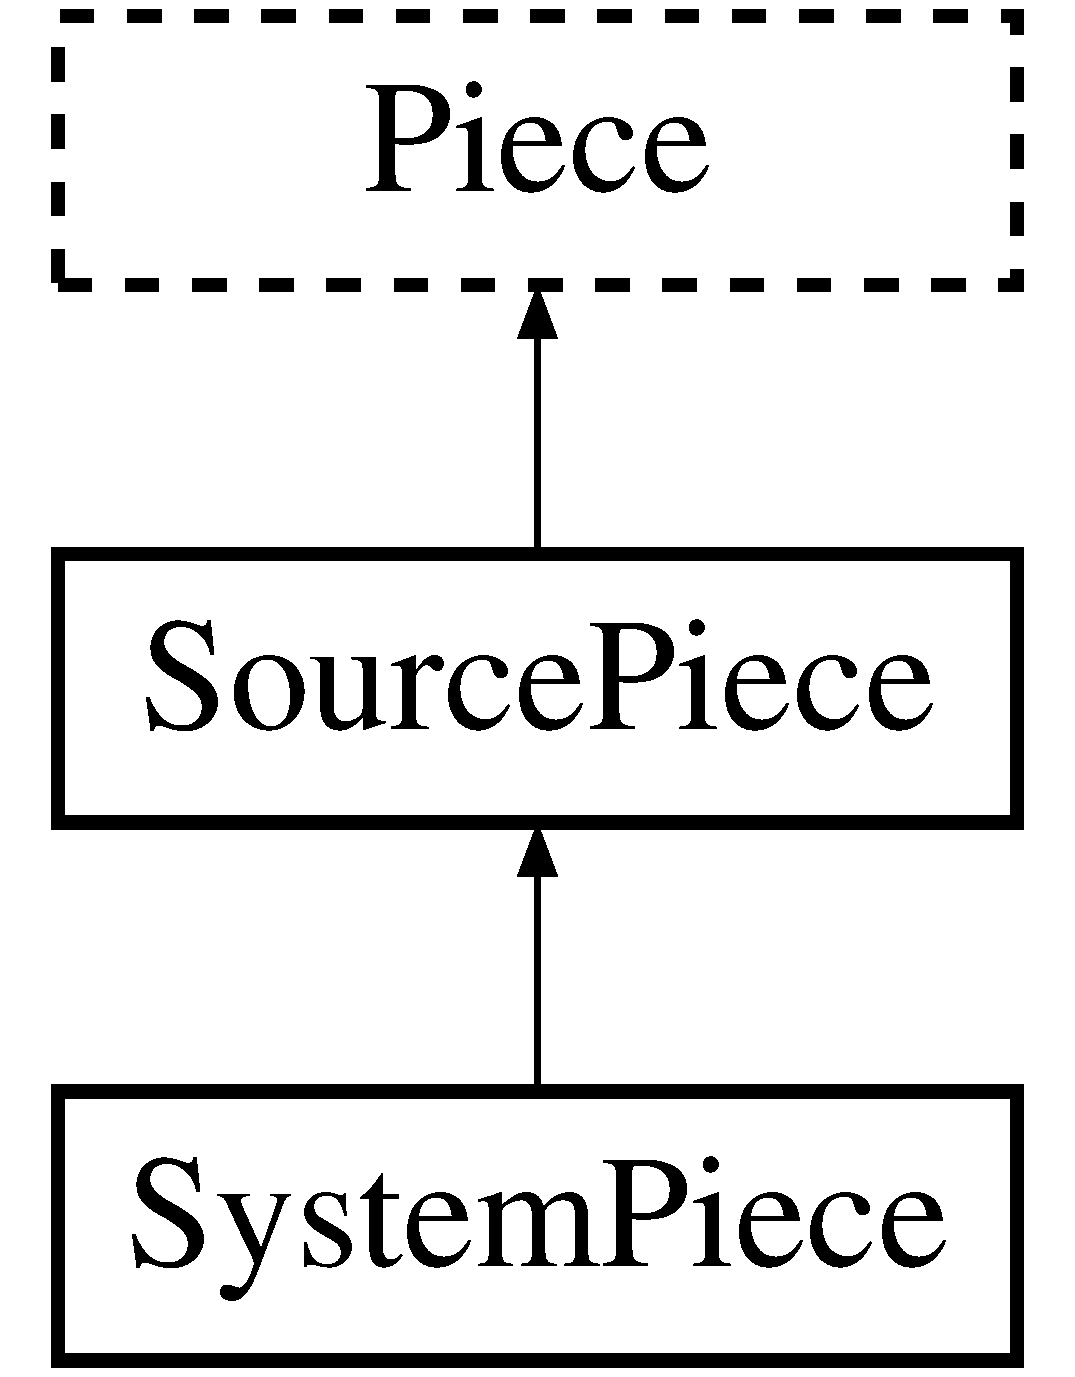
\includegraphics[height=3.000000cm]{classSourcePiece}
\end{center}
\end{figure}
\subsection*{Public Member Functions}
\begin{DoxyCompactItemize}
\item 
\hyperlink{structCoordinate}{Coordinate} \hyperlink{classSourcePiece_a15e950d71f3d178d0d585246deedc6b8}{get\-Source} ()
\begin{DoxyCompactList}\small\item\em Returns the source. \end{DoxyCompactList}\item 
void \hyperlink{classSourcePiece_a8f9733cc1e7f75aad92c12d84d8710e2}{set\-Source} (\hyperlink{structCoordinate}{Coordinate} \hyperlink{classSourcePiece_a9c04073192af496ceaf536dfb334a718}{source})
\begin{DoxyCompactList}\small\item\em Sets the source coordinate. \end{DoxyCompactList}\item 
\hyperlink{classSourcePiece_abdff14565936734507eac75bb4f929ea}{Source\-Piece} (\hyperlink{classPlayer}{Player} $\ast$\hyperlink{classPiece_a43beac3b5268343b9f7e575d637eda98}{owner}, \hyperlink{structCoordinate}{Coordinate} \hyperlink{classSourcePiece_a9c04073192af496ceaf536dfb334a718}{source})
\end{DoxyCompactItemize}
\subsection*{Protected Attributes}
\begin{DoxyCompactItemize}
\item 
\hyperlink{structCoordinate}{Coordinate} \hyperlink{classSourcePiece_a9c04073192af496ceaf536dfb334a718}{source}
\begin{DoxyCompactList}\small\item\em \hyperlink{structCoordinate}{Coordinate} containing the source. \end{DoxyCompactList}\end{DoxyCompactItemize}
\subsection*{Additional Inherited Members}


\subsection{Detailed Description}
A \hyperlink{classPiece}{Piece} with a source. \begin{DoxyAuthor}{Author}
Ian Duffy 
\end{DoxyAuthor}


Definition at line 9 of file Source\-Piece.\-h.



\subsection{Constructor \& Destructor Documentation}
\hypertarget{classSourcePiece_abdff14565936734507eac75bb4f929ea}{\index{Source\-Piece@{Source\-Piece}!Source\-Piece@{Source\-Piece}}
\index{Source\-Piece@{Source\-Piece}!SourcePiece@{Source\-Piece}}
\subsubsection[{Source\-Piece}]{\setlength{\rightskip}{0pt plus 5cm}Source\-Piece\-::\-Source\-Piece (
\begin{DoxyParamCaption}
\item[{{\bf Player} $\ast$}]{owner, }
\item[{{\bf Coordinate}}]{source}
\end{DoxyParamCaption}
)}}\label{classSourcePiece_abdff14565936734507eac75bb4f929ea}
A \hyperlink{classPiece}{Piece} with a source. \begin{DoxyAuthor}{Author}
Ian Duffy 
\end{DoxyAuthor}


Definition at line 6 of file Source\-Piece.\-cpp.



\subsection{Member Function Documentation}
\hypertarget{classSourcePiece_a15e950d71f3d178d0d585246deedc6b8}{\index{Source\-Piece@{Source\-Piece}!get\-Source@{get\-Source}}
\index{get\-Source@{get\-Source}!SourcePiece@{Source\-Piece}}
\subsubsection[{get\-Source}]{\setlength{\rightskip}{0pt plus 5cm}{\bf Coordinate} Source\-Piece\-::get\-Source (
\begin{DoxyParamCaption}
{}
\end{DoxyParamCaption}
)}}\label{classSourcePiece_a15e950d71f3d178d0d585246deedc6b8}


Returns the source. 



Definition at line 12 of file Source\-Piece.\-cpp.

\hypertarget{classSourcePiece_a8f9733cc1e7f75aad92c12d84d8710e2}{\index{Source\-Piece@{Source\-Piece}!set\-Source@{set\-Source}}
\index{set\-Source@{set\-Source}!SourcePiece@{Source\-Piece}}
\subsubsection[{set\-Source}]{\setlength{\rightskip}{0pt plus 5cm}void Source\-Piece\-::set\-Source (
\begin{DoxyParamCaption}
\item[{{\bf Coordinate}}]{source}
\end{DoxyParamCaption}
)}}\label{classSourcePiece_a8f9733cc1e7f75aad92c12d84d8710e2}


Sets the source coordinate. 



Definition at line 17 of file Source\-Piece.\-cpp.



\subsection{Field Documentation}
\hypertarget{classSourcePiece_a9c04073192af496ceaf536dfb334a718}{\index{Source\-Piece@{Source\-Piece}!source@{source}}
\index{source@{source}!SourcePiece@{Source\-Piece}}
\subsubsection[{source}]{\setlength{\rightskip}{0pt plus 5cm}{\bf Coordinate} Source\-Piece\-::source\hspace{0.3cm}{\ttfamily [protected]}}}\label{classSourcePiece_a9c04073192af496ceaf536dfb334a718}


\hyperlink{structCoordinate}{Coordinate} containing the source. 



Definition at line 12 of file Source\-Piece.\-h.



The documentation for this class was generated from the following files\-:\begin{DoxyCompactItemize}
\item 
\hyperlink{SourcePiece_8h}{Source\-Piece.\-h}\item 
\hyperlink{SourcePiece_8cpp}{Source\-Piece.\-cpp}\end{DoxyCompactItemize}

\hypertarget{classSquare}{\section{Square Class Reference}
\label{classSquare}\index{Square@{Square}}
}


{\ttfamily \#include $<$Square.\-h$>$}

\subsection*{Public Member Functions}
\begin{DoxyCompactItemize}
\item 
bool \hyperlink{classSquare_a8839d897e85342bc9ccd0c3c8ae37ac1}{add\-Piece} (int \hyperlink{classPlayer}{Player}, \hyperlink{classPiece}{Piece} $\ast$piece)
\item 
string \hyperlink{classSquare_aa2d3fa7c91fef0ab75b657fff84a0e5d}{get\-End} ()
\item 
int \hyperlink{classSquare_a61e01113ed501094f077facc98247834}{get\-Identifier} ()
\item 
\hyperlink{classPiece}{Piece} $\ast$ \hyperlink{classSquare_ae679e5dba819d52e03d96e4d6b192aba}{get\-Piece} (int player)
\item 
\hyperlink{structCoordinate}{Coordinate} \hyperlink{classSquare_a49a097184b5773dbdac054aba5eaf556}{get\-Position} ()
\item 
string \hyperlink{classSquare_a950cc5ee3db1236f953b2b54a7eb2aad}{get\-Start} ()
\item 
bool \hyperlink{classSquare_a875e971657b4670b121837d80f247626}{has\-Piece} ()
\item 
bool \hyperlink{classSquare_a767fa41efec1594d87ae7b47854ea8f1}{has\-Piece\-Owned\-By} (int player)
\item 
bool \hyperlink{classSquare_aa549b2d293165c7978b21f7d26f58fb2}{remove\-Piece} (int player)
\item 
\hyperlink{classSquare_a3dc7ff9aefc2725172b5d3153973d243}{Square} ()
\item 
\hyperlink{classSquare_ae66f3039b28e813bcdc832bbe1f5ddcf}{Square} (int \hyperlink{classSquare_a564b1f548b3be90a32c0dfd045de1187}{identifier}, string \hyperlink{classSquare_ab8661c5b8e8026d074cf11c9e6634d18}{start}, string \hyperlink{classSquare_a419b11e7d6cac76bfbc89c9b1ad111f2}{end}, int \hyperlink{classSquare_ae6bded80423341335f9dd86c189955c0}{amount\-Of\-Players}, \hyperlink{structCoordinate}{Coordinate} \hyperlink{classSquare_a08e99afd7be993cd1cbb50f4716e95ff}{position})
\end{DoxyCompactItemize}
\subsection*{Protected Attributes}
\begin{DoxyCompactItemize}
\item 
int \hyperlink{classSquare_ae6bded80423341335f9dd86c189955c0}{amount\-Of\-Players}
\item 
string \hyperlink{classSquare_a419b11e7d6cac76bfbc89c9b1ad111f2}{end}
\item 
int \hyperlink{classSquare_a564b1f548b3be90a32c0dfd045de1187}{identifier}
\item 
int \hyperlink{classSquare_a61b6be58fcaec7b02aa82158cf9ac6fe}{number\-Of\-Occupants}
\item 
vector$<$ \hyperlink{classPiece}{Piece} $\ast$ $>$ \hyperlink{classSquare_a144124544a38dc3e81ff702191c1c627}{pieces}
\item 
\hyperlink{structCoordinate}{Coordinate} \hyperlink{classSquare_a08e99afd7be993cd1cbb50f4716e95ff}{position}
\item 
string \hyperlink{classSquare_ab8661c5b8e8026d074cf11c9e6634d18}{start}
\end{DoxyCompactItemize}
\subsection*{Friends}
\begin{DoxyCompactItemize}
\item 
ostream \& \hyperlink{classSquare_a1cef282cd4504e20e1687a571e9cf943}{operator$<$$<$} (ostream \&out, const \hyperlink{classSquare}{Square} \&square)
\begin{DoxyCompactList}\small\item\em Overrides the insert operator for a square. \end{DoxyCompactList}\end{DoxyCompactItemize}


\subsection{Detailed Description}


Definition at line 14 of file Square.\-h.



\subsection{Constructor \& Destructor Documentation}
\hypertarget{classSquare_a3dc7ff9aefc2725172b5d3153973d243}{\index{Square@{Square}!Square@{Square}}
\index{Square@{Square}!Square@{Square}}
\subsubsection[{Square}]{\setlength{\rightskip}{0pt plus 5cm}Square\-::\-Square (
\begin{DoxyParamCaption}
{}
\end{DoxyParamCaption}
)}}\label{classSquare_a3dc7ff9aefc2725172b5d3153973d243}


Definition at line 3 of file Square.\-cpp.

\hypertarget{classSquare_ae66f3039b28e813bcdc832bbe1f5ddcf}{\index{Square@{Square}!Square@{Square}}
\index{Square@{Square}!Square@{Square}}
\subsubsection[{Square}]{\setlength{\rightskip}{0pt plus 5cm}Square\-::\-Square (
\begin{DoxyParamCaption}
\item[{int}]{identifier, }
\item[{string}]{start, }
\item[{string}]{end, }
\item[{int}]{amount\-Of\-Players, }
\item[{{\bf Coordinate}}]{position}
\end{DoxyParamCaption}
)}}\label{classSquare_ae66f3039b28e813bcdc832bbe1f5ddcf}


Definition at line 5 of file Square.\-cpp.



\subsection{Member Function Documentation}
\hypertarget{classSquare_a8839d897e85342bc9ccd0c3c8ae37ac1}{\index{Square@{Square}!add\-Piece@{add\-Piece}}
\index{add\-Piece@{add\-Piece}!Square@{Square}}
\subsubsection[{add\-Piece}]{\setlength{\rightskip}{0pt plus 5cm}bool Square\-::add\-Piece (
\begin{DoxyParamCaption}
\item[{int}]{Player, }
\item[{{\bf Piece} $\ast$}]{piece}
\end{DoxyParamCaption}
)}}\label{classSquare_a8839d897e85342bc9ccd0c3c8ae37ac1}


Definition at line 19 of file Square.\-cpp.

\hypertarget{classSquare_aa2d3fa7c91fef0ab75b657fff84a0e5d}{\index{Square@{Square}!get\-End@{get\-End}}
\index{get\-End@{get\-End}!Square@{Square}}
\subsubsection[{get\-End}]{\setlength{\rightskip}{0pt plus 5cm}string Square\-::get\-End (
\begin{DoxyParamCaption}
{}
\end{DoxyParamCaption}
)}}\label{classSquare_aa2d3fa7c91fef0ab75b657fff84a0e5d}


Definition at line 60 of file Square.\-cpp.

\hypertarget{classSquare_a61e01113ed501094f077facc98247834}{\index{Square@{Square}!get\-Identifier@{get\-Identifier}}
\index{get\-Identifier@{get\-Identifier}!Square@{Square}}
\subsubsection[{get\-Identifier}]{\setlength{\rightskip}{0pt plus 5cm}int Square\-::get\-Identifier (
\begin{DoxyParamCaption}
{}
\end{DoxyParamCaption}
)}}\label{classSquare_a61e01113ed501094f077facc98247834}


Definition at line 41 of file Square.\-cpp.

\hypertarget{classSquare_ae679e5dba819d52e03d96e4d6b192aba}{\index{Square@{Square}!get\-Piece@{get\-Piece}}
\index{get\-Piece@{get\-Piece}!Square@{Square}}
\subsubsection[{get\-Piece}]{\setlength{\rightskip}{0pt plus 5cm}{\bf Piece} $\ast$ Square\-::get\-Piece (
\begin{DoxyParamCaption}
\item[{int}]{player}
\end{DoxyParamCaption}
)}}\label{classSquare_ae679e5dba819d52e03d96e4d6b192aba}


Definition at line 52 of file Square.\-cpp.

\hypertarget{classSquare_a49a097184b5773dbdac054aba5eaf556}{\index{Square@{Square}!get\-Position@{get\-Position}}
\index{get\-Position@{get\-Position}!Square@{Square}}
\subsubsection[{get\-Position}]{\setlength{\rightskip}{0pt plus 5cm}{\bf Coordinate} Square\-::get\-Position (
\begin{DoxyParamCaption}
{}
\end{DoxyParamCaption}
)}}\label{classSquare_a49a097184b5773dbdac054aba5eaf556}


Definition at line 37 of file Square.\-cpp.

\hypertarget{classSquare_a950cc5ee3db1236f953b2b54a7eb2aad}{\index{Square@{Square}!get\-Start@{get\-Start}}
\index{get\-Start@{get\-Start}!Square@{Square}}
\subsubsection[{get\-Start}]{\setlength{\rightskip}{0pt plus 5cm}string Square\-::get\-Start (
\begin{DoxyParamCaption}
{}
\end{DoxyParamCaption}
)}}\label{classSquare_a950cc5ee3db1236f953b2b54a7eb2aad}


Definition at line 56 of file Square.\-cpp.

\hypertarget{classSquare_a875e971657b4670b121837d80f247626}{\index{Square@{Square}!has\-Piece@{has\-Piece}}
\index{has\-Piece@{has\-Piece}!Square@{Square}}
\subsubsection[{has\-Piece}]{\setlength{\rightskip}{0pt plus 5cm}bool Square\-::has\-Piece (
\begin{DoxyParamCaption}
{}
\end{DoxyParamCaption}
)}}\label{classSquare_a875e971657b4670b121837d80f247626}


Definition at line 15 of file Square.\-cpp.

\hypertarget{classSquare_a767fa41efec1594d87ae7b47854ea8f1}{\index{Square@{Square}!has\-Piece\-Owned\-By@{has\-Piece\-Owned\-By}}
\index{has\-Piece\-Owned\-By@{has\-Piece\-Owned\-By}!Square@{Square}}
\subsubsection[{has\-Piece\-Owned\-By}]{\setlength{\rightskip}{0pt plus 5cm}bool Square\-::has\-Piece\-Owned\-By (
\begin{DoxyParamCaption}
\item[{int}]{player}
\end{DoxyParamCaption}
)}}\label{classSquare_a767fa41efec1594d87ae7b47854ea8f1}


Definition at line 45 of file Square.\-cpp.

\hypertarget{classSquare_aa549b2d293165c7978b21f7d26f58fb2}{\index{Square@{Square}!remove\-Piece@{remove\-Piece}}
\index{remove\-Piece@{remove\-Piece}!Square@{Square}}
\subsubsection[{remove\-Piece}]{\setlength{\rightskip}{0pt plus 5cm}bool Square\-::remove\-Piece (
\begin{DoxyParamCaption}
\item[{int}]{player}
\end{DoxyParamCaption}
)}}\label{classSquare_aa549b2d293165c7978b21f7d26f58fb2}


Definition at line 31 of file Square.\-cpp.



\subsection{Friends And Related Function Documentation}
\hypertarget{classSquare_a1cef282cd4504e20e1687a571e9cf943}{\index{Square@{Square}!operator$<$$<$@{operator$<$$<$}}
\index{operator$<$$<$@{operator$<$$<$}!Square@{Square}}
\subsubsection[{operator$<$$<$}]{\setlength{\rightskip}{0pt plus 5cm}ostream\& operator$<$$<$ (
\begin{DoxyParamCaption}
\item[{ostream \&}]{out, }
\item[{const {\bf Square} \&}]{square}
\end{DoxyParamCaption}
)\hspace{0.3cm}{\ttfamily [friend]}}}\label{classSquare_a1cef282cd4504e20e1687a571e9cf943}


Overrides the insert operator for a square. 



Definition at line 54 of file Game.\-cpp.



\subsection{Field Documentation}
\hypertarget{classSquare_ae6bded80423341335f9dd86c189955c0}{\index{Square@{Square}!amount\-Of\-Players@{amount\-Of\-Players}}
\index{amount\-Of\-Players@{amount\-Of\-Players}!Square@{Square}}
\subsubsection[{amount\-Of\-Players}]{\setlength{\rightskip}{0pt plus 5cm}int Square\-::amount\-Of\-Players\hspace{0.3cm}{\ttfamily [protected]}}}\label{classSquare_ae6bded80423341335f9dd86c189955c0}


Definition at line 20 of file Square.\-h.

\hypertarget{classSquare_a419b11e7d6cac76bfbc89c9b1ad111f2}{\index{Square@{Square}!end@{end}}
\index{end@{end}!Square@{Square}}
\subsubsection[{end}]{\setlength{\rightskip}{0pt plus 5cm}string Square\-::end\hspace{0.3cm}{\ttfamily [protected]}}}\label{classSquare_a419b11e7d6cac76bfbc89c9b1ad111f2}


Definition at line 23 of file Square.\-h.

\hypertarget{classSquare_a564b1f548b3be90a32c0dfd045de1187}{\index{Square@{Square}!identifier@{identifier}}
\index{identifier@{identifier}!Square@{Square}}
\subsubsection[{identifier}]{\setlength{\rightskip}{0pt plus 5cm}int Square\-::identifier\hspace{0.3cm}{\ttfamily [protected]}}}\label{classSquare_a564b1f548b3be90a32c0dfd045de1187}


Definition at line 19 of file Square.\-h.

\hypertarget{classSquare_a61b6be58fcaec7b02aa82158cf9ac6fe}{\index{Square@{Square}!number\-Of\-Occupants@{number\-Of\-Occupants}}
\index{number\-Of\-Occupants@{number\-Of\-Occupants}!Square@{Square}}
\subsubsection[{number\-Of\-Occupants}]{\setlength{\rightskip}{0pt plus 5cm}int Square\-::number\-Of\-Occupants\hspace{0.3cm}{\ttfamily [protected]}}}\label{classSquare_a61b6be58fcaec7b02aa82158cf9ac6fe}


Definition at line 21 of file Square.\-h.

\hypertarget{classSquare_a144124544a38dc3e81ff702191c1c627}{\index{Square@{Square}!pieces@{pieces}}
\index{pieces@{pieces}!Square@{Square}}
\subsubsection[{pieces}]{\setlength{\rightskip}{0pt plus 5cm}vector$<${\bf Piece} $\ast$$>$ Square\-::pieces\hspace{0.3cm}{\ttfamily [protected]}}}\label{classSquare_a144124544a38dc3e81ff702191c1c627}


Definition at line 24 of file Square.\-h.

\hypertarget{classSquare_a08e99afd7be993cd1cbb50f4716e95ff}{\index{Square@{Square}!position@{position}}
\index{position@{position}!Square@{Square}}
\subsubsection[{position}]{\setlength{\rightskip}{0pt plus 5cm}{\bf Coordinate} Square\-::position\hspace{0.3cm}{\ttfamily [protected]}}}\label{classSquare_a08e99afd7be993cd1cbb50f4716e95ff}


Definition at line 25 of file Square.\-h.

\hypertarget{classSquare_ab8661c5b8e8026d074cf11c9e6634d18}{\index{Square@{Square}!start@{start}}
\index{start@{start}!Square@{Square}}
\subsubsection[{start}]{\setlength{\rightskip}{0pt plus 5cm}string Square\-::start\hspace{0.3cm}{\ttfamily [protected]}}}\label{classSquare_ab8661c5b8e8026d074cf11c9e6634d18}


Definition at line 22 of file Square.\-h.



The documentation for this class was generated from the following files\-:\begin{DoxyCompactItemize}
\item 
\hyperlink{Square_8h}{Square.\-h}\item 
\hyperlink{Square_8cpp}{Square.\-cpp}\end{DoxyCompactItemize}

\hypertarget{classSystemPiece}{\section{System\-Piece Class Reference}
\label{classSystemPiece}\index{System\-Piece@{System\-Piece}}
}


{\ttfamily \#include $<$System\-Piece.\-h$>$}

Inheritance diagram for System\-Piece\-:\begin{figure}[H]
\begin{center}
\leavevmode
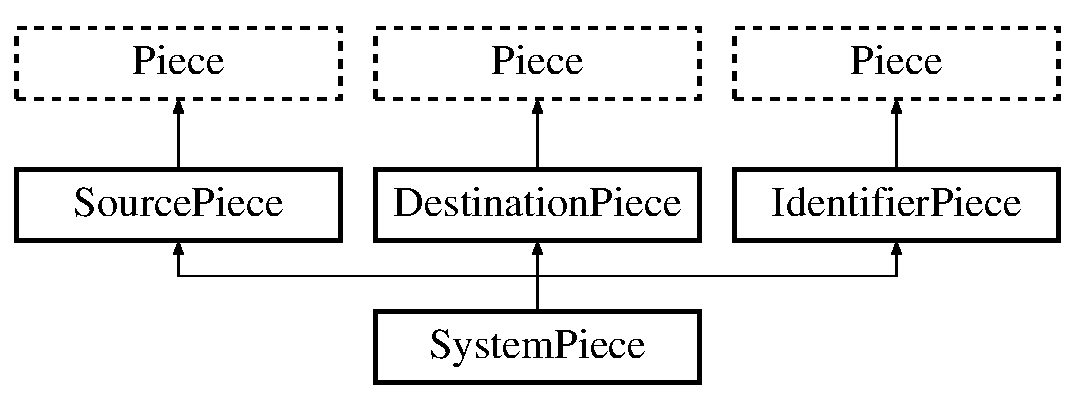
\includegraphics[height=3.000000cm]{classSystemPiece}
\end{center}
\end{figure}
\subsection*{Public Member Functions}
\begin{DoxyCompactItemize}
\item 
\hyperlink{classSystemPiece_a5af9dda7ff0a7a5a6a0262a9d80ab956}{System\-Piece} (\hyperlink{classPlayer}{Player} $\ast$\hyperlink{classPiece_a43beac3b5268343b9f7e575d637eda98}{owner}, \hyperlink{structCoordinate}{Coordinate} \hyperlink{classSourcePiece_a9c04073192af496ceaf536dfb334a718}{source}, \hyperlink{structCoordinate}{Coordinate} \hyperlink{classDestinationPiece_acd3a864aa8c242f3b8b7d27195a2d879}{destination}, int \hyperlink{classIdentifierPiece_aab84613c911d8d7c269b9636ce6faa36}{identifier})
\end{DoxyCompactItemize}
\subsection*{Additional Inherited Members}


\subsection{Detailed Description}
A piece with made up of a \hyperlink{classSourcePiece}{Source\-Piece}, \hyperlink{classDestinationPiece}{Destination\-Piece} and \hyperlink{classIdentifierPiece}{Identifier\-Piece}. \begin{DoxyAuthor}{Author}
Ian Duffy 

Darren Brogan 
\end{DoxyAuthor}


Definition at line 13 of file System\-Piece.\-h.



\subsection{Constructor \& Destructor Documentation}
\hypertarget{classSystemPiece_a5af9dda7ff0a7a5a6a0262a9d80ab956}{\index{System\-Piece@{System\-Piece}!System\-Piece@{System\-Piece}}
\index{System\-Piece@{System\-Piece}!SystemPiece@{System\-Piece}}
\subsubsection[{System\-Piece}]{\setlength{\rightskip}{0pt plus 5cm}System\-Piece\-::\-System\-Piece (
\begin{DoxyParamCaption}
\item[{{\bf Player} $\ast$}]{owner, }
\item[{{\bf Coordinate}}]{source, }
\item[{{\bf Coordinate}}]{destination, }
\item[{int}]{identifier}
\end{DoxyParamCaption}
)}}\label{classSystemPiece_a5af9dda7ff0a7a5a6a0262a9d80ab956}
A piece with made up of a \hyperlink{classSourcePiece}{Source\-Piece}, \hyperlink{classDestinationPiece}{Destination\-Piece} and \hyperlink{classIdentifierPiece}{Identifier\-Piece}. \begin{DoxyAuthor}{Author}
Ian Duffy 

Darren Brogan 
\end{DoxyAuthor}


Definition at line 7 of file System\-Piece.\-cpp.



The documentation for this class was generated from the following files\-:\begin{DoxyCompactItemize}
\item 
\hyperlink{SystemPiece_8h}{System\-Piece.\-h}\item 
\hyperlink{SystemPiece_8cpp}{System\-Piece.\-cpp}\end{DoxyCompactItemize}

\chapter{File Documentation}
\hypertarget{Checkers_8cpp}{\section{Checkers.\-cpp File Reference}
\label{Checkers_8cpp}\index{Checkers.\-cpp@{Checkers.\-cpp}}
}
{\ttfamily \#include \char`\"{}Checkers.\-h\char`\"{}}\\*

\hypertarget{Checkers_8h}{\section{Checkers.\-h File Reference}
\label{Checkers_8h}\index{Checkers.\-h@{Checkers.\-h}}
}
{\ttfamily \#include \char`\"{}Game.\-h\char`\"{}}\\*
\subsection*{Data Structures}
\begin{DoxyCompactItemize}
\item 
class \hyperlink{classCheckers}{Checkers}
\end{DoxyCompactItemize}

\hypertarget{Colors_8h}{\section{Colors.\-h File Reference}
\label{Colors_8h}\index{Colors.\-h@{Colors.\-h}}
}
\subsection*{Macros}
\begin{DoxyCompactItemize}
\item 
\#define \hyperlink{Colors_8h_ac04a55099d9d2fdf09eeb11b6edda922}{B\-B\-L\-A\-C\-K}~\char`\"{}\char`\"{}
\item 
\#define \hyperlink{Colors_8h_a4c97932a8044a468113b4e1dadc5fa08}{B\-B\-L\-U\-E}~\char`\"{}\char`\"{}
\item 
\#define \hyperlink{Colors_8h_aa94753e91817ff9a941a7f0b2544f957}{B\-C\-Y\-A\-N}~\char`\"{}\char`\"{}
\item 
\#define \hyperlink{Colors_8h_ae1a8523e23479cb4ea0037864dca5434}{B\-G\-R\-E\-E\-N}~\char`\"{}\char`\"{}
\item 
\#define \hyperlink{Colors_8h_a9c8c1e4e648327ce326b9bba579a4e41}{B\-M\-A\-G\-E\-N\-T\-A}~\char`\"{}\char`\"{}
\item 
\#define \hyperlink{Colors_8h_a6cdb0db424dd3bca247b151d6edd526e}{B\-O\-R\-A\-N\-G\-E}~\char`\"{}\char`\"{}
\item 
\#define \hyperlink{Colors_8h_a2adb4c9e293ac446897ccfac5a52d6c2}{B\-R\-E\-D}~\char`\"{}\char`\"{}
\item 
\#define \hyperlink{Colors_8h_af92883b29f19ec3c5ca5b1f4c45d01a2}{B\-V\-I\-O\-L\-E\-T}~\char`\"{}\char`\"{}
\item 
\#define \hyperlink{Colors_8h_ac9b496a3875fbea1a5254c660ba36c58}{B\-W\-H\-I\-T\-E}~\char`\"{}\char`\"{}
\item 
\#define \hyperlink{Colors_8h_a755f95481f7549a35580011e24323833}{B\-Y\-E\-L\-L\-O\-W}~\char`\"{}\char`\"{}
\item 
\#define \hyperlink{Colors_8h_af05ab189f2b42d8724023c5da7288110}{F\-B\-L\-A\-C\-K}~\char`\"{}\char`\"{}
\item 
\#define \hyperlink{Colors_8h_ac7bbc3e4b0858dfeca51ba3c15a13a48}{F\-B\-L\-U\-E}~\char`\"{}\char`\"{}
\item 
\#define \hyperlink{Colors_8h_a0ea2a482bdf8513e4a50dae67d972b0a}{F\-C\-Y\-A\-N}~\char`\"{}\char`\"{}
\item 
\#define \hyperlink{Colors_8h_a205f1ecfd8eae9b29ff8a8fbe5f5b4b4}{F\-G\-R\-E\-E\-N}~\char`\"{}\char`\"{}
\item 
\#define \hyperlink{Colors_8h_a62b512f5b602e5368fc1333291254207}{F\-M\-A\-G\-E\-N\-T\-A}~\char`\"{}\char`\"{}
\item 
\#define \hyperlink{Colors_8h_a8965927e93af144bee00b7a9179b99bd}{F\-O\-R\-A\-N\-G\-E}~\char`\"{}\char`\"{}
\item 
\#define \hyperlink{Colors_8h_ab41c5ea389c93bdcab9fea2f2946eaaa}{F\-R\-E\-D}~\char`\"{}\char`\"{}
\item 
\#define \hyperlink{Colors_8h_a97b5a6c871e27678d2f2a632bc8262ee}{F\-V\-I\-O\-L\-E\-T}~\char`\"{}\char`\"{}
\item 
\#define \hyperlink{Colors_8h_aa959b776116c67f49182bd7e7c42a231}{F\-W\-H\-I\-T\-E}~\char`\"{}\char`\"{}
\item 
\#define \hyperlink{Colors_8h_a6504ad628ed3640dfc115f1fcafaa299}{F\-Y\-E\-L\-L\-O\-W}~\char`\"{}\char`\"{}
\end{DoxyCompactItemize}


\subsection{Macro Definition Documentation}
\hypertarget{Colors_8h_ac04a55099d9d2fdf09eeb11b6edda922}{\index{Colors.\-h@{Colors.\-h}!B\-B\-L\-A\-C\-K@{B\-B\-L\-A\-C\-K}}
\index{B\-B\-L\-A\-C\-K@{B\-B\-L\-A\-C\-K}!Colors.h@{Colors.\-h}}
\subsubsection[{B\-B\-L\-A\-C\-K}]{\setlength{\rightskip}{0pt plus 5cm}\#define B\-B\-L\-A\-C\-K~\char`\"{}\char`\"{}}}\label{Colors_8h_ac04a55099d9d2fdf09eeb11b6edda922}


Definition at line 37 of file Colors.\-h.

\hypertarget{Colors_8h_a4c97932a8044a468113b4e1dadc5fa08}{\index{Colors.\-h@{Colors.\-h}!B\-B\-L\-U\-E@{B\-B\-L\-U\-E}}
\index{B\-B\-L\-U\-E@{B\-B\-L\-U\-E}!Colors.h@{Colors.\-h}}
\subsubsection[{B\-B\-L\-U\-E}]{\setlength{\rightskip}{0pt plus 5cm}\#define B\-B\-L\-U\-E~\char`\"{}\char`\"{}}}\label{Colors_8h_a4c97932a8044a468113b4e1dadc5fa08}


Definition at line 44 of file Colors.\-h.

\hypertarget{Colors_8h_aa94753e91817ff9a941a7f0b2544f957}{\index{Colors.\-h@{Colors.\-h}!B\-C\-Y\-A\-N@{B\-C\-Y\-A\-N}}
\index{B\-C\-Y\-A\-N@{B\-C\-Y\-A\-N}!Colors.h@{Colors.\-h}}
\subsubsection[{B\-C\-Y\-A\-N}]{\setlength{\rightskip}{0pt plus 5cm}\#define B\-C\-Y\-A\-N~\char`\"{}\char`\"{}}}\label{Colors_8h_aa94753e91817ff9a941a7f0b2544f957}


Definition at line 45 of file Colors.\-h.

\hypertarget{Colors_8h_ae1a8523e23479cb4ea0037864dca5434}{\index{Colors.\-h@{Colors.\-h}!B\-G\-R\-E\-E\-N@{B\-G\-R\-E\-E\-N}}
\index{B\-G\-R\-E\-E\-N@{B\-G\-R\-E\-E\-N}!Colors.h@{Colors.\-h}}
\subsubsection[{B\-G\-R\-E\-E\-N}]{\setlength{\rightskip}{0pt plus 5cm}\#define B\-G\-R\-E\-E\-N~\char`\"{}\char`\"{}}}\label{Colors_8h_ae1a8523e23479cb4ea0037864dca5434}


Definition at line 46 of file Colors.\-h.

\hypertarget{Colors_8h_a9c8c1e4e648327ce326b9bba579a4e41}{\index{Colors.\-h@{Colors.\-h}!B\-M\-A\-G\-E\-N\-T\-A@{B\-M\-A\-G\-E\-N\-T\-A}}
\index{B\-M\-A\-G\-E\-N\-T\-A@{B\-M\-A\-G\-E\-N\-T\-A}!Colors.h@{Colors.\-h}}
\subsubsection[{B\-M\-A\-G\-E\-N\-T\-A}]{\setlength{\rightskip}{0pt plus 5cm}\#define B\-M\-A\-G\-E\-N\-T\-A~\char`\"{}\char`\"{}}}\label{Colors_8h_a9c8c1e4e648327ce326b9bba579a4e41}


Definition at line 42 of file Colors.\-h.

\hypertarget{Colors_8h_a6cdb0db424dd3bca247b151d6edd526e}{\index{Colors.\-h@{Colors.\-h}!B\-O\-R\-A\-N\-G\-E@{B\-O\-R\-A\-N\-G\-E}}
\index{B\-O\-R\-A\-N\-G\-E@{B\-O\-R\-A\-N\-G\-E}!Colors.h@{Colors.\-h}}
\subsubsection[{B\-O\-R\-A\-N\-G\-E}]{\setlength{\rightskip}{0pt plus 5cm}\#define B\-O\-R\-A\-N\-G\-E~\char`\"{}\char`\"{}}}\label{Colors_8h_a6cdb0db424dd3bca247b151d6edd526e}


Definition at line 40 of file Colors.\-h.

\hypertarget{Colors_8h_a2adb4c9e293ac446897ccfac5a52d6c2}{\index{Colors.\-h@{Colors.\-h}!B\-R\-E\-D@{B\-R\-E\-D}}
\index{B\-R\-E\-D@{B\-R\-E\-D}!Colors.h@{Colors.\-h}}
\subsubsection[{B\-R\-E\-D}]{\setlength{\rightskip}{0pt plus 5cm}\#define B\-R\-E\-D~\char`\"{}\char`\"{}}}\label{Colors_8h_a2adb4c9e293ac446897ccfac5a52d6c2}


Definition at line 41 of file Colors.\-h.

\hypertarget{Colors_8h_af92883b29f19ec3c5ca5b1f4c45d01a2}{\index{Colors.\-h@{Colors.\-h}!B\-V\-I\-O\-L\-E\-T@{B\-V\-I\-O\-L\-E\-T}}
\index{B\-V\-I\-O\-L\-E\-T@{B\-V\-I\-O\-L\-E\-T}!Colors.h@{Colors.\-h}}
\subsubsection[{B\-V\-I\-O\-L\-E\-T}]{\setlength{\rightskip}{0pt plus 5cm}\#define B\-V\-I\-O\-L\-E\-T~\char`\"{}\char`\"{}}}\label{Colors_8h_af92883b29f19ec3c5ca5b1f4c45d01a2}


Definition at line 43 of file Colors.\-h.

\hypertarget{Colors_8h_ac9b496a3875fbea1a5254c660ba36c58}{\index{Colors.\-h@{Colors.\-h}!B\-W\-H\-I\-T\-E@{B\-W\-H\-I\-T\-E}}
\index{B\-W\-H\-I\-T\-E@{B\-W\-H\-I\-T\-E}!Colors.h@{Colors.\-h}}
\subsubsection[{B\-W\-H\-I\-T\-E}]{\setlength{\rightskip}{0pt plus 5cm}\#define B\-W\-H\-I\-T\-E~\char`\"{}\char`\"{}}}\label{Colors_8h_ac9b496a3875fbea1a5254c660ba36c58}


Definition at line 38 of file Colors.\-h.

\hypertarget{Colors_8h_a755f95481f7549a35580011e24323833}{\index{Colors.\-h@{Colors.\-h}!B\-Y\-E\-L\-L\-O\-W@{B\-Y\-E\-L\-L\-O\-W}}
\index{B\-Y\-E\-L\-L\-O\-W@{B\-Y\-E\-L\-L\-O\-W}!Colors.h@{Colors.\-h}}
\subsubsection[{B\-Y\-E\-L\-L\-O\-W}]{\setlength{\rightskip}{0pt plus 5cm}\#define B\-Y\-E\-L\-L\-O\-W~\char`\"{}\char`\"{}}}\label{Colors_8h_a755f95481f7549a35580011e24323833}


Definition at line 39 of file Colors.\-h.

\hypertarget{Colors_8h_af05ab189f2b42d8724023c5da7288110}{\index{Colors.\-h@{Colors.\-h}!F\-B\-L\-A\-C\-K@{F\-B\-L\-A\-C\-K}}
\index{F\-B\-L\-A\-C\-K@{F\-B\-L\-A\-C\-K}!Colors.h@{Colors.\-h}}
\subsubsection[{F\-B\-L\-A\-C\-K}]{\setlength{\rightskip}{0pt plus 5cm}\#define F\-B\-L\-A\-C\-K~\char`\"{}\char`\"{}}}\label{Colors_8h_af05ab189f2b42d8724023c5da7288110}


Definition at line 50 of file Colors.\-h.

\hypertarget{Colors_8h_ac7bbc3e4b0858dfeca51ba3c15a13a48}{\index{Colors.\-h@{Colors.\-h}!F\-B\-L\-U\-E@{F\-B\-L\-U\-E}}
\index{F\-B\-L\-U\-E@{F\-B\-L\-U\-E}!Colors.h@{Colors.\-h}}
\subsubsection[{F\-B\-L\-U\-E}]{\setlength{\rightskip}{0pt plus 5cm}\#define F\-B\-L\-U\-E~\char`\"{}\char`\"{}}}\label{Colors_8h_ac7bbc3e4b0858dfeca51ba3c15a13a48}


Definition at line 57 of file Colors.\-h.

\hypertarget{Colors_8h_a0ea2a482bdf8513e4a50dae67d972b0a}{\index{Colors.\-h@{Colors.\-h}!F\-C\-Y\-A\-N@{F\-C\-Y\-A\-N}}
\index{F\-C\-Y\-A\-N@{F\-C\-Y\-A\-N}!Colors.h@{Colors.\-h}}
\subsubsection[{F\-C\-Y\-A\-N}]{\setlength{\rightskip}{0pt plus 5cm}\#define F\-C\-Y\-A\-N~\char`\"{}\char`\"{}}}\label{Colors_8h_a0ea2a482bdf8513e4a50dae67d972b0a}


Definition at line 58 of file Colors.\-h.

\hypertarget{Colors_8h_a205f1ecfd8eae9b29ff8a8fbe5f5b4b4}{\index{Colors.\-h@{Colors.\-h}!F\-G\-R\-E\-E\-N@{F\-G\-R\-E\-E\-N}}
\index{F\-G\-R\-E\-E\-N@{F\-G\-R\-E\-E\-N}!Colors.h@{Colors.\-h}}
\subsubsection[{F\-G\-R\-E\-E\-N}]{\setlength{\rightskip}{0pt plus 5cm}\#define F\-G\-R\-E\-E\-N~\char`\"{}\char`\"{}}}\label{Colors_8h_a205f1ecfd8eae9b29ff8a8fbe5f5b4b4}


Definition at line 59 of file Colors.\-h.

\hypertarget{Colors_8h_a62b512f5b602e5368fc1333291254207}{\index{Colors.\-h@{Colors.\-h}!F\-M\-A\-G\-E\-N\-T\-A@{F\-M\-A\-G\-E\-N\-T\-A}}
\index{F\-M\-A\-G\-E\-N\-T\-A@{F\-M\-A\-G\-E\-N\-T\-A}!Colors.h@{Colors.\-h}}
\subsubsection[{F\-M\-A\-G\-E\-N\-T\-A}]{\setlength{\rightskip}{0pt plus 5cm}\#define F\-M\-A\-G\-E\-N\-T\-A~\char`\"{}\char`\"{}}}\label{Colors_8h_a62b512f5b602e5368fc1333291254207}


Definition at line 55 of file Colors.\-h.

\hypertarget{Colors_8h_a8965927e93af144bee00b7a9179b99bd}{\index{Colors.\-h@{Colors.\-h}!F\-O\-R\-A\-N\-G\-E@{F\-O\-R\-A\-N\-G\-E}}
\index{F\-O\-R\-A\-N\-G\-E@{F\-O\-R\-A\-N\-G\-E}!Colors.h@{Colors.\-h}}
\subsubsection[{F\-O\-R\-A\-N\-G\-E}]{\setlength{\rightskip}{0pt plus 5cm}\#define F\-O\-R\-A\-N\-G\-E~\char`\"{}\char`\"{}}}\label{Colors_8h_a8965927e93af144bee00b7a9179b99bd}


Definition at line 53 of file Colors.\-h.

\hypertarget{Colors_8h_ab41c5ea389c93bdcab9fea2f2946eaaa}{\index{Colors.\-h@{Colors.\-h}!F\-R\-E\-D@{F\-R\-E\-D}}
\index{F\-R\-E\-D@{F\-R\-E\-D}!Colors.h@{Colors.\-h}}
\subsubsection[{F\-R\-E\-D}]{\setlength{\rightskip}{0pt plus 5cm}\#define F\-R\-E\-D~\char`\"{}\char`\"{}}}\label{Colors_8h_ab41c5ea389c93bdcab9fea2f2946eaaa}


Definition at line 54 of file Colors.\-h.

\hypertarget{Colors_8h_a97b5a6c871e27678d2f2a632bc8262ee}{\index{Colors.\-h@{Colors.\-h}!F\-V\-I\-O\-L\-E\-T@{F\-V\-I\-O\-L\-E\-T}}
\index{F\-V\-I\-O\-L\-E\-T@{F\-V\-I\-O\-L\-E\-T}!Colors.h@{Colors.\-h}}
\subsubsection[{F\-V\-I\-O\-L\-E\-T}]{\setlength{\rightskip}{0pt plus 5cm}\#define F\-V\-I\-O\-L\-E\-T~\char`\"{}\char`\"{}}}\label{Colors_8h_a97b5a6c871e27678d2f2a632bc8262ee}


Definition at line 56 of file Colors.\-h.

\hypertarget{Colors_8h_aa959b776116c67f49182bd7e7c42a231}{\index{Colors.\-h@{Colors.\-h}!F\-W\-H\-I\-T\-E@{F\-W\-H\-I\-T\-E}}
\index{F\-W\-H\-I\-T\-E@{F\-W\-H\-I\-T\-E}!Colors.h@{Colors.\-h}}
\subsubsection[{F\-W\-H\-I\-T\-E}]{\setlength{\rightskip}{0pt plus 5cm}\#define F\-W\-H\-I\-T\-E~\char`\"{}\char`\"{}}}\label{Colors_8h_aa959b776116c67f49182bd7e7c42a231}


Definition at line 51 of file Colors.\-h.

\hypertarget{Colors_8h_a6504ad628ed3640dfc115f1fcafaa299}{\index{Colors.\-h@{Colors.\-h}!F\-Y\-E\-L\-L\-O\-W@{F\-Y\-E\-L\-L\-O\-W}}
\index{F\-Y\-E\-L\-L\-O\-W@{F\-Y\-E\-L\-L\-O\-W}!Colors.h@{Colors.\-h}}
\subsubsection[{F\-Y\-E\-L\-L\-O\-W}]{\setlength{\rightskip}{0pt plus 5cm}\#define F\-Y\-E\-L\-L\-O\-W~\char`\"{}\char`\"{}}}\label{Colors_8h_a6504ad628ed3640dfc115f1fcafaa299}


Definition at line 52 of file Colors.\-h.


\hypertarget{ConnectFour_8cpp}{\section{Connect\-Four.\-cpp File Reference}
\label{ConnectFour_8cpp}\index{Connect\-Four.\-cpp@{Connect\-Four.\-cpp}}
}
{\ttfamily \#include \char`\"{}Connect\-Four.\-h\char`\"{}}\\*

\hypertarget{ConnectFour_8h}{\section{Connect\-Four.\-h File Reference}
\label{ConnectFour_8h}\index{Connect\-Four.\-h@{Connect\-Four.\-h}}
}
{\ttfamily \#include $<$string$>$}\\*
{\ttfamily \#include $<$iostream$>$}\\*
{\ttfamily \#include \char`\"{}Game.\-h\char`\"{}}\\*
{\ttfamily \#include \char`\"{}Square.\-h\char`\"{}}\\*
{\ttfamily \#include \char`\"{}Player.\-h\char`\"{}}\\*
\subsection*{Data Structures}
\begin{DoxyCompactItemize}
\item 
class \hyperlink{classConnectFour}{Connect\-Four}
\end{DoxyCompactItemize}
\subsection*{Macros}
\begin{DoxyCompactItemize}
\item 
\#define \hyperlink{ConnectFour_8h_a1f09123e56cf7ba4f4f5c38b21e62428}{C\-O\-N\-N\-C\-T\-F\-O\-U\-R}
\end{DoxyCompactItemize}


\subsection{Macro Definition Documentation}
\hypertarget{ConnectFour_8h_a1f09123e56cf7ba4f4f5c38b21e62428}{\index{Connect\-Four.\-h@{Connect\-Four.\-h}!C\-O\-N\-N\-C\-T\-F\-O\-U\-R@{C\-O\-N\-N\-C\-T\-F\-O\-U\-R}}
\index{C\-O\-N\-N\-C\-T\-F\-O\-U\-R@{C\-O\-N\-N\-C\-T\-F\-O\-U\-R}!ConnectFour.h@{Connect\-Four.\-h}}
\subsubsection[{C\-O\-N\-N\-C\-T\-F\-O\-U\-R}]{\setlength{\rightskip}{0pt plus 5cm}\#define C\-O\-N\-N\-C\-T\-F\-O\-U\-R}}\label{ConnectFour_8h_a1f09123e56cf7ba4f4f5c38b21e62428}


Definition at line 2 of file Connect\-Four.\-h.


\hypertarget{Coordinate_8cpp}{\section{Coordinate.\-cpp File Reference}
\label{Coordinate_8cpp}\index{Coordinate.\-cpp@{Coordinate.\-cpp}}
}
{\ttfamily \#include \char`\"{}Coordinate.\-h\char`\"{}}\\*

\hypertarget{Coordinate_8h}{\section{Coordinate.\-h File Reference}
\label{Coordinate_8h}\index{Coordinate.\-h@{Coordinate.\-h}}
}
\subsection*{Data Structures}
\begin{DoxyCompactItemize}
\item 
struct \hyperlink{structCoordinate}{Coordinate}
\end{DoxyCompactItemize}

\hypertarget{DECLARATION_8md}{\section{D\-E\-C\-L\-A\-R\-A\-T\-I\-O\-N.\-md File Reference}
\label{DECLARATION_8md}\index{D\-E\-C\-L\-A\-R\-A\-T\-I\-O\-N.\-md@{D\-E\-C\-L\-A\-R\-A\-T\-I\-O\-N.\-md}}
}

\hypertarget{DestinationPiece_8cpp}{\section{Destination\-Piece.\-cpp File Reference}
\label{DestinationPiece_8cpp}\index{Destination\-Piece.\-cpp@{Destination\-Piece.\-cpp}}
}
{\ttfamily \#include \char`\"{}Destination\-Piece.\-h\char`\"{}}\\*

\hypertarget{DestinationPiece_8h}{\section{Destination\-Piece.\-h File Reference}
\label{DestinationPiece_8h}\index{Destination\-Piece.\-h@{Destination\-Piece.\-h}}
}
{\ttfamily \#include \char`\"{}Piece.\-h\char`\"{}}\\*
\subsection*{Data Structures}
\begin{DoxyCompactItemize}
\item 
class \hyperlink{classDestinationPiece}{Destination\-Piece}
\end{DoxyCompactItemize}

\hypertarget{Game_8cpp}{\section{Game.\-cpp File Reference}
\label{Game_8cpp}\index{Game.\-cpp@{Game.\-cpp}}
}
{\ttfamily \#include \char`\"{}Game.\-h\char`\"{}}\\*
\subsection*{Functions}
\begin{DoxyCompactItemize}
\item 
ostream \& \hyperlink{Game_8cpp_abdfecfa2a12a51344ff1b0a4293b9703}{operator$<$$<$} (ostream \&os, const \hyperlink{classSquare}{Square} \&square)
\begin{DoxyCompactList}\small\item\em Overrides the insert operator for a square. \end{DoxyCompactList}\item 
ostream \& \hyperlink{Game_8cpp_a9f608da6a114112a40fd6243c63dc5fa}{operator$<$$<$} (ostream \&os, const \hyperlink{classPiece}{Piece} \&piece)
\begin{DoxyCompactList}\small\item\em Overrides the insert operator for a piece. \end{DoxyCompactList}\end{DoxyCompactItemize}


\subsection{Function Documentation}
\hypertarget{Game_8cpp_abdfecfa2a12a51344ff1b0a4293b9703}{\index{Game.\-cpp@{Game.\-cpp}!operator$<$$<$@{operator$<$$<$}}
\index{operator$<$$<$@{operator$<$$<$}!Game.cpp@{Game.\-cpp}}
\subsubsection[{operator$<$$<$}]{\setlength{\rightskip}{0pt plus 5cm}ostream\& operator$<$$<$ (
\begin{DoxyParamCaption}
\item[{ostream \&}]{os, }
\item[{const {\bf Square} \&}]{square}
\end{DoxyParamCaption}
)}}\label{Game_8cpp_abdfecfa2a12a51344ff1b0a4293b9703}


Overrides the insert operator for a square. 



Definition at line 54 of file Game.\-cpp.

\hypertarget{Game_8cpp_a9f608da6a114112a40fd6243c63dc5fa}{\index{Game.\-cpp@{Game.\-cpp}!operator$<$$<$@{operator$<$$<$}}
\index{operator$<$$<$@{operator$<$$<$}!Game.cpp@{Game.\-cpp}}
\subsubsection[{operator$<$$<$}]{\setlength{\rightskip}{0pt plus 5cm}ostream\& operator$<$$<$ (
\begin{DoxyParamCaption}
\item[{ostream \&}]{os, }
\item[{const {\bf Piece} \&}]{piece}
\end{DoxyParamCaption}
)}}\label{Game_8cpp_a9f608da6a114112a40fd6243c63dc5fa}


Overrides the insert operator for a piece. 



Definition at line 66 of file Game.\-cpp.


\hypertarget{Game_8h}{\section{Game.\-h File Reference}
\label{Game_8h}\index{Game.\-h@{Game.\-h}}
}
{\ttfamily \#include $<$string$>$}\\*
{\ttfamily \#include $<$vector$>$}\\*
{\ttfamily \#include $<$iostream$>$}\\*
{\ttfamily \#include $<$cstdlib$>$}\\*
{\ttfamily \#include $<$cstdio$>$}\\*
{\ttfamily \#include \char`\"{}Square.\-h\char`\"{}}\\*
{\ttfamily \#include \char`\"{}Player.\-h\char`\"{}}\\*
{\ttfamily \#include \char`\"{}Colors.\-h\char`\"{}}\\*
\subsection*{Data Structures}
\begin{DoxyCompactItemize}
\item 
class \hyperlink{classGame}{Game}
\end{DoxyCompactItemize}

\hypertarget{IdentifierPiece_8cpp}{\section{Identifier\-Piece.\-cpp File Reference}
\label{IdentifierPiece_8cpp}\index{Identifier\-Piece.\-cpp@{Identifier\-Piece.\-cpp}}
}
{\ttfamily \#include \char`\"{}Identifier\-Piece.\-h\char`\"{}}\\*

\hypertarget{IdentifierPiece_8h}{\section{Identifier\-Piece.\-h File Reference}
\label{IdentifierPiece_8h}\index{Identifier\-Piece.\-h@{Identifier\-Piece.\-h}}
}
{\ttfamily \#include \char`\"{}Piece.\-h\char`\"{}}\\*
\subsection*{Data Structures}
\begin{DoxyCompactItemize}
\item 
class \hyperlink{classIdentifierPiece}{Identifier\-Piece}
\end{DoxyCompactItemize}

\hypertarget{main_8cpp}{\section{main.\-cpp File Reference}
\label{main_8cpp}\index{main.\-cpp@{main.\-cpp}}
}
{\ttfamily \#include $<$iostream$>$}\\*
{\ttfamily \#include $<$iomanip$>$}\\*
{\ttfamily \#include \char`\"{}Checkers.\-h\char`\"{}}\\*
{\ttfamily \#include \char`\"{}Connect\-Four.\-h\char`\"{}}\\*
{\ttfamily \#include \char`\"{}Snakes\-And\-Ladders.\-h\char`\"{}}\\*
{\ttfamily \#include \char`\"{}Colors.\-h\char`\"{}}\\*
\subsection*{Functions}
\begin{DoxyCompactItemize}
\item 
void \hyperlink{main_8cpp_ac8af80a653557a0722584cee4f2fde51}{border} (int width)
\begin{DoxyCompactList}\small\item\em Print border. \end{DoxyCompactList}\item 
int \hyperlink{main_8cpp_ae66f6b31b5ad750f1fe042a706a4e3d4}{main} ()
\end{DoxyCompactItemize}


\subsection{Function Documentation}
\hypertarget{main_8cpp_ac8af80a653557a0722584cee4f2fde51}{\index{main.\-cpp@{main.\-cpp}!border@{border}}
\index{border@{border}!main.cpp@{main.\-cpp}}
\subsubsection[{border}]{\setlength{\rightskip}{0pt plus 5cm}void border (
\begin{DoxyParamCaption}
\item[{int}]{width}
\end{DoxyParamCaption}
)}}\label{main_8cpp_ac8af80a653557a0722584cee4f2fde51}


Print border. 



Definition at line 73 of file main.\-cpp.

\hypertarget{main_8cpp_ae66f6b31b5ad750f1fe042a706a4e3d4}{\index{main.\-cpp@{main.\-cpp}!main@{main}}
\index{main@{main}!main.cpp@{main.\-cpp}}
\subsubsection[{main}]{\setlength{\rightskip}{0pt plus 5cm}int main (
\begin{DoxyParamCaption}
{}
\end{DoxyParamCaption}
)}}\label{main_8cpp_ae66f6b31b5ad750f1fe042a706a4e3d4}
Print out the titles of each game

Create a vector of pointers to hold the locations of each game

games\mbox{[}4\mbox{]} = new Reversi();

Ensure that the selection is valid

Launch selected game 

Definition at line 14 of file main.\-cpp.


\hypertarget{Piece_8cpp}{\section{Piece.\-cpp File Reference}
\label{Piece_8cpp}\index{Piece.\-cpp@{Piece.\-cpp}}
}
{\ttfamily \#include \char`\"{}Piece.\-h\char`\"{}}\\*
{\ttfamily \#include \char`\"{}Player.\-h\char`\"{}}\\*

\hypertarget{Piece_8h}{\section{Piece.\-h File Reference}
\label{Piece_8h}\index{Piece.\-h@{Piece.\-h}}
}
{\ttfamily \#include $<$iostream$>$}\\*
{\ttfamily \#include \char`\"{}Coordinate.\-h\char`\"{}}\\*
\subsection*{Data Structures}
\begin{DoxyCompactItemize}
\item 
class \hyperlink{classPiece}{Piece}
\end{DoxyCompactItemize}

\hypertarget{Player_8cpp}{\section{Player.\-cpp File Reference}
\label{Player_8cpp}\index{Player.\-cpp@{Player.\-cpp}}
}
{\ttfamily \#include \char`\"{}Player.\-h\char`\"{}}\\*
{\ttfamily \#include \char`\"{}Piece.\-h\char`\"{}}\\*

\hypertarget{Player_8h}{\section{Player.\-h File Reference}
\label{Player_8h}\index{Player.\-h@{Player.\-h}}
}
{\ttfamily \#include $<$string$>$}\\*
{\ttfamily \#include $<$vector$>$}\\*
{\ttfamily \#include \char`\"{}Coordinate.\-h\char`\"{}}\\*
\subsection*{Data Structures}
\begin{DoxyCompactItemize}
\item 
class \hyperlink{classPlayer}{Player}
\end{DoxyCompactItemize}

\hypertarget{README_8md}{\section{R\-E\-A\-D\-M\-E.\-md File Reference}
\label{README_8md}\index{R\-E\-A\-D\-M\-E.\-md@{R\-E\-A\-D\-M\-E.\-md}}
}

\hypertarget{SnakesAndLadders_8cpp}{\section{Snakes\-And\-Ladders.\-cpp File Reference}
\label{SnakesAndLadders_8cpp}\index{Snakes\-And\-Ladders.\-cpp@{Snakes\-And\-Ladders.\-cpp}}
}
{\ttfamily \#include \char`\"{}Snakes\-And\-Ladders.\-h\char`\"{}}\\*
\subsection*{Typedefs}
\begin{DoxyCompactItemize}
\item 
typedef \hyperlink{structCoordinate}{Coordinate} \hyperlink{SnakesAndLadders_8cpp_a49cbd0dde8da44412dd11cfdafcf69d5}{Coord}
\item 
typedef \hyperlink{classDestinationPiece}{Destination\-Piece} \hyperlink{SnakesAndLadders_8cpp_a033aa9efe52c4fd9b6f29fb5c3adc44a}{Dest\-Piece}
\item 
typedef \hyperlink{classIdentifierPiece}{Identifier\-Piece} \hyperlink{SnakesAndLadders_8cpp_a910e22346b7111781f645fa3614fbb5e}{I\-D\-Piece}
\item 
typedef \hyperlink{classSnakesAndLaddersPlayer}{Snakes\-And\-Ladders\-Player} \hyperlink{SnakesAndLadders_8cpp_af1bc8eaffdf81e73df605fb0ea591ea1}{S\-L\-Player}
\item 
typedef \hyperlink{classSourcePiece}{Source\-Piece} \hyperlink{SnakesAndLadders_8cpp_a85eca5611b73504030077490d3eac597}{Src\-Piece}
\end{DoxyCompactItemize}


\subsection{Typedef Documentation}
\hypertarget{SnakesAndLadders_8cpp_a49cbd0dde8da44412dd11cfdafcf69d5}{\index{Snakes\-And\-Ladders.\-cpp@{Snakes\-And\-Ladders.\-cpp}!Coord@{Coord}}
\index{Coord@{Coord}!SnakesAndLadders.cpp@{Snakes\-And\-Ladders.\-cpp}}
\subsubsection[{Coord}]{\setlength{\rightskip}{0pt plus 5cm}typedef {\bf Coordinate} {\bf Coord}}}\label{SnakesAndLadders_8cpp_a49cbd0dde8da44412dd11cfdafcf69d5}


Definition at line 13 of file Snakes\-And\-Ladders.\-cpp.

\hypertarget{SnakesAndLadders_8cpp_a033aa9efe52c4fd9b6f29fb5c3adc44a}{\index{Snakes\-And\-Ladders.\-cpp@{Snakes\-And\-Ladders.\-cpp}!Dest\-Piece@{Dest\-Piece}}
\index{Dest\-Piece@{Dest\-Piece}!SnakesAndLadders.cpp@{Snakes\-And\-Ladders.\-cpp}}
\subsubsection[{Dest\-Piece}]{\setlength{\rightskip}{0pt plus 5cm}typedef {\bf Destination\-Piece} {\bf Dest\-Piece}}}\label{SnakesAndLadders_8cpp_a033aa9efe52c4fd9b6f29fb5c3adc44a}


Definition at line 11 of file Snakes\-And\-Ladders.\-cpp.

\hypertarget{SnakesAndLadders_8cpp_a910e22346b7111781f645fa3614fbb5e}{\index{Snakes\-And\-Ladders.\-cpp@{Snakes\-And\-Ladders.\-cpp}!I\-D\-Piece@{I\-D\-Piece}}
\index{I\-D\-Piece@{I\-D\-Piece}!SnakesAndLadders.cpp@{Snakes\-And\-Ladders.\-cpp}}
\subsubsection[{I\-D\-Piece}]{\setlength{\rightskip}{0pt plus 5cm}typedef {\bf Identifier\-Piece} {\bf I\-D\-Piece}}}\label{SnakesAndLadders_8cpp_a910e22346b7111781f645fa3614fbb5e}


Definition at line 12 of file Snakes\-And\-Ladders.\-cpp.

\hypertarget{SnakesAndLadders_8cpp_af1bc8eaffdf81e73df605fb0ea591ea1}{\index{Snakes\-And\-Ladders.\-cpp@{Snakes\-And\-Ladders.\-cpp}!S\-L\-Player@{S\-L\-Player}}
\index{S\-L\-Player@{S\-L\-Player}!SnakesAndLadders.cpp@{Snakes\-And\-Ladders.\-cpp}}
\subsubsection[{S\-L\-Player}]{\setlength{\rightskip}{0pt plus 5cm}typedef {\bf Snakes\-And\-Ladders\-Player} {\bf S\-L\-Player}}}\label{SnakesAndLadders_8cpp_af1bc8eaffdf81e73df605fb0ea591ea1}


Definition at line 9 of file Snakes\-And\-Ladders.\-cpp.

\hypertarget{SnakesAndLadders_8cpp_a85eca5611b73504030077490d3eac597}{\index{Snakes\-And\-Ladders.\-cpp@{Snakes\-And\-Ladders.\-cpp}!Src\-Piece@{Src\-Piece}}
\index{Src\-Piece@{Src\-Piece}!SnakesAndLadders.cpp@{Snakes\-And\-Ladders.\-cpp}}
\subsubsection[{Src\-Piece}]{\setlength{\rightskip}{0pt plus 5cm}typedef {\bf Source\-Piece} {\bf Src\-Piece}}}\label{SnakesAndLadders_8cpp_a85eca5611b73504030077490d3eac597}


Definition at line 10 of file Snakes\-And\-Ladders.\-cpp.


\hypertarget{SnakesAndLadders_8h}{\section{Snakes\-And\-Ladders.\-h File Reference}
\label{SnakesAndLadders_8h}\index{Snakes\-And\-Ladders.\-h@{Snakes\-And\-Ladders.\-h}}
}
{\ttfamily \#include \char`\"{}Game.\-h\char`\"{}}\\*
{\ttfamily \#include \char`\"{}Snakes\-And\-Ladders\-Player.\-h\char`\"{}}\\*
{\ttfamily \#include \char`\"{}Source\-Piece.\-h\char`\"{}}\\*
{\ttfamily \#include \char`\"{}System\-Piece.\-h\char`\"{}}\\*
\subsection*{Data Structures}
\begin{DoxyCompactItemize}
\item 
class \hyperlink{classSnakesAndLadders}{Snakes\-And\-Ladders}
\end{DoxyCompactItemize}

\hypertarget{SnakesAndLaddersPlayer_8cpp}{\section{Snakes\-And\-Ladders\-Player.\-cpp File Reference}
\label{SnakesAndLaddersPlayer_8cpp}\index{Snakes\-And\-Ladders\-Player.\-cpp@{Snakes\-And\-Ladders\-Player.\-cpp}}
}
{\ttfamily \#include \char`\"{}Snakes\-And\-Ladders\-Player.\-h\char`\"{}}\\*

\hypertarget{SnakesAndLaddersPlayer_8h}{\section{Snakes\-And\-Ladders\-Player.\-h File Reference}
\label{SnakesAndLaddersPlayer_8h}\index{Snakes\-And\-Ladders\-Player.\-h@{Snakes\-And\-Ladders\-Player.\-h}}
}
{\ttfamily \#include \char`\"{}Player.\-h\char`\"{}}\\*
\subsection*{Data Structures}
\begin{DoxyCompactItemize}
\item 
class \hyperlink{classSnakesAndLaddersPlayer}{Snakes\-And\-Ladders\-Player}
\end{DoxyCompactItemize}

\hypertarget{SourcePiece_8cpp}{\section{Source\-Piece.\-cpp File Reference}
\label{SourcePiece_8cpp}\index{Source\-Piece.\-cpp@{Source\-Piece.\-cpp}}
}
{\ttfamily \#include \char`\"{}Source\-Piece.\-h\char`\"{}}\\*

\hypertarget{SourcePiece_8h}{\section{Source\-Piece.\-h File Reference}
\label{SourcePiece_8h}\index{Source\-Piece.\-h@{Source\-Piece.\-h}}
}
{\ttfamily \#include \char`\"{}Piece.\-h\char`\"{}}\\*
\subsection*{Data Structures}
\begin{DoxyCompactItemize}
\item 
class \hyperlink{classSourcePiece}{Source\-Piece}
\end{DoxyCompactItemize}

\hypertarget{Square_8cpp}{\section{Square.\-cpp File Reference}
\label{Square_8cpp}\index{Square.\-cpp@{Square.\-cpp}}
}
{\ttfamily \#include \char`\"{}Square.\-h\char`\"{}}\\*

\hypertarget{Square_8h}{\section{Square.\-h File Reference}
\label{Square_8h}\index{Square.\-h@{Square.\-h}}
}
{\ttfamily \#include $<$string$>$}\\*
{\ttfamily \#include $<$vector$>$}\\*
{\ttfamily \#include \char`\"{}Piece.\-h\char`\"{}}\\*
{\ttfamily \#include \char`\"{}Player.\-h\char`\"{}}\\*
{\ttfamily \#include \char`\"{}Coordinate.\-h\char`\"{}}\\*
\subsection*{Data Structures}
\begin{DoxyCompactItemize}
\item 
class \hyperlink{classSquare}{Square}
\end{DoxyCompactItemize}

\hypertarget{SystemPiece_8cpp}{\section{System\-Piece.\-cpp File Reference}
\label{SystemPiece_8cpp}\index{System\-Piece.\-cpp@{System\-Piece.\-cpp}}
}
{\ttfamily \#include \char`\"{}System\-Piece.\-h\char`\"{}}\\*

\hypertarget{SystemPiece_8h}{\section{System\-Piece.\-h File Reference}
\label{SystemPiece_8h}\index{System\-Piece.\-h@{System\-Piece.\-h}}
}
{\ttfamily \#include \char`\"{}Piece.\-h\char`\"{}}\\*
{\ttfamily \#include \char`\"{}Source\-Piece.\-h\char`\"{}}\\*
{\ttfamily \#include \char`\"{}Destination\-Piece.\-h\char`\"{}}\\*
{\ttfamily \#include \char`\"{}Identifier\-Piece.\-h\char`\"{}}\\*
\subsection*{Data Structures}
\begin{DoxyCompactItemize}
\item 
class \hyperlink{classSystemPiece}{System\-Piece}
\end{DoxyCompactItemize}

\addcontentsline{toc}{part}{Index}
\printindex
\end{document}
